\chapter{Plane Geometry}

\section{Overview: Representation and Operations of Points}

\begin{itembox}[l]{Overview}
We encounter opportunities to handle geometric problems with computers in various situations. Here, I would like to introduce the basics of dealing with geometric problems (please take a specialized course to learn more). For example, let's try to represent familiar concepts such as parallelism and inside/outside of a figure using the tool of "signed area of a triangle." Even for simple geometric concepts for humans, there are cases where non-intuitive methods are suitable when describing them as programs. Also, since we are dealing with floating-point numbers (\texttt{double}, etc.), it is necessary to pay attention to errors.
\end{itembox}

When representing points on a plane in C or C++, for example, there is a method using structures (\pcaojbook[pp.~365--(Chapter 16)]). In this material, to make it a little easier, we will represent them as complex numbers as follows.
\subsection{Representation of Points Using Complex Numbers}

\paragraph{Representation Using Complex Numbers in C++}
In C++, the \eindex{complex} type in the standard library is used. (The real part \texttt{real()} corresponds to \texttt{x}, and the imaginary part \texttt{imag()} corresponds to \texttt{y}):
\begin{center}
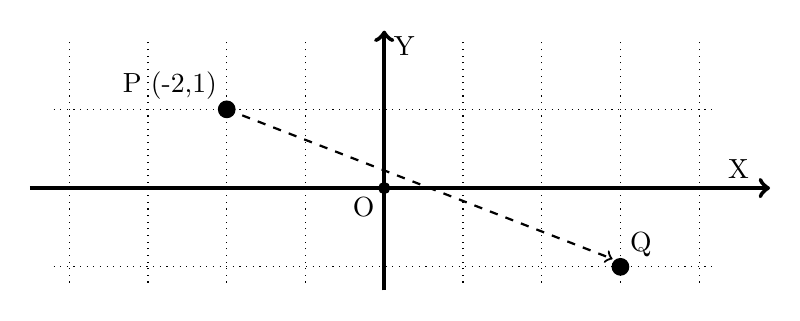
\begin{tikzpicture}
\coordinate (O) at (0,0);
\coordinate (P) at (-2,1);
\coordinate (Q) at (3,-1);
\draw [step=1cm,dotted] (-4.2,-1.2) grid (4.2,1.9);
\draw [->,ultra thick] (-4.5,0) -- (4.9,0);
\draw [->,ultra thick] (0,-1.3) -- (0,2.0);
\node [above] at (4.5,0) {X};
\node [right] at (0,1.8) {Y};
\draw [fill=black] (O) circle (2pt);
\node [below left] at (0,0) {O};
\draw [fill=black] (P) circle (3pt);
\node [above left] at (P) {P (-2,1)};
\draw [fill=black] (Q) circle (3pt);
\node [above right] at (Q) {Q};
\draw [->,thick,dashed] (P) -- (2.9,-0.9);
\end{tikzpicture}
\end{center}

\begin{cbox}[emph={complex,real,imag}]
#include <complex>
#include <cmath>
typedef complex<double> xy_t;
xy_t P(-2, 1), Q; // Initialization
cout << P << endl; // (for debug) display
cout << P.real() << endl; // x coordinate
cout << P.imag() << endl; // y coordinate
Q = P + xy_t(5, -2); // Point Q is the position of point P translated by (5,-2)
Q *= xy_t(cos(a), sin(a)); // Rotate point Q around the origin by a (radians)
cout << abs(P) << endl; // Length of vector OP
cout << norm(P) << endl; // \texttt{norm(P) = abs(P)}${}^2$
\end{cbox}

\paragraph{Representation Using Complex Numbers in C} Although the use of C is not recommended in this material, it is included here for the sake of the notes mentioned later.

In the case of C (gcc or C99):
\begin{purecbox}[emph={complex,creal,cimag}]
#include <complex.h>
#include <math.h>
complex a = 0.0 + 1.0I; // Initialization
complex b = cos(3.14/4) + sin(3.14/4)*I;
printf("
a *= b; // Multiplication
printf("
\end{purecbox}

\begin{debugbox}{Caution about Forgetting Multiplication Symbols}
  When calculating the product of the number \texttt{5} and the variable \texttt{k}, write \texttt{5*k}; writing \texttt{5k} will result in a compilation error. However, for the characters \texttt{i,j,I,J}, notations such as \texttt{5j} are interpreted as the imaginary unit above and do not cause a compilation error. When displayed with \texttt{cout}, it is cast to \texttt{bool} and displayed as \texttt{1}. This can be difficult to find if you are not aware of it.
\end{debugbox}

\medskip

\paragraph{Representation Using Complex Numbers in Python} In Python3, complex numbers \texttt{complex} can be used in almost the same way. For details, please check \texttt{help(complex)} or \texttt{help(cmath)}.
\begin{pybox}[emph={real,imag,complex}]
import cmath
import math
P = complex(-2,1) # \texttt{(-2+1j)} is also acceptable
print(P)
print(P.real)     # Real part
print(P.imag)     # Imaginary part
Q = P + complex(5,-2)     # Translation
Q *= complex(math.cos(a), math.sin(a))     # Rotation
print(abs(P))     # Length
\end{pybox}
\subsection{Frequently Used Operations}

\begin{center}
\begin{tabular}{c@{\hspace{5em}}c}
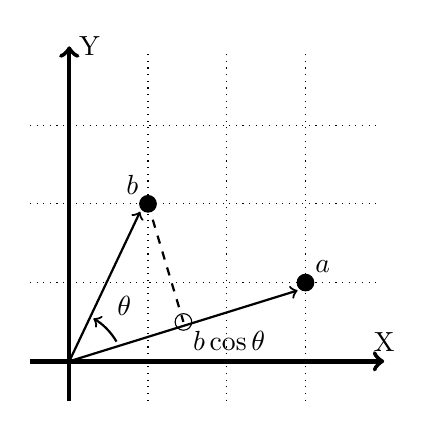
\begin{tikzpicture}
\coordinate (O) at (0,0);
\coordinate (A) at (3,1);
\coordinate (B) at (1,2);
\coordinate (BcosT) at (1.45,0.5);
\draw [step=1cm,dotted] (-0.5,-0.5) grid (3.9,3.9);
\draw [->,ultra thick] (-0.5,0) -- (4,0);
\draw [->,ultra thick] (0,-0.5) -- (0,4);
\node [above] at (4,0) {X};
\node [right] at (0,4) {Y};
\draw [fill=black] (A) circle (3pt);
\node [above right] at (A) {$a$};
\draw [fill=black] (B) circle (3pt);
\node [above left] at (B) {$b$};
\draw [] (BcosT) circle (3pt);
\node [below right] at (BcosT) {$b\cos\theta$};
\draw [->,thick] (O) -- (2.9,0.9);
\draw [->,thick] (O) -- (0.9,1.9);
\draw [->,thick] (0.6,0.25) arc (30:60:0.8);
\draw [thick,dashed] (B) -- (BcosT);
\node at (0.7,0.7) {$\theta$};
\end{tikzpicture}
&
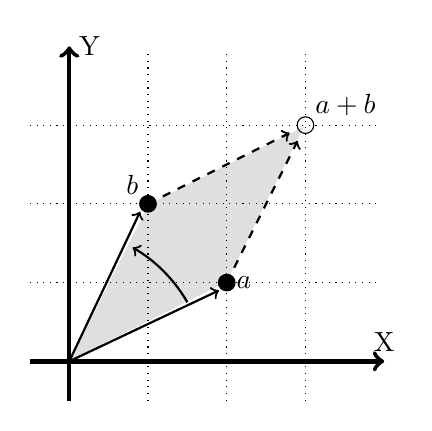
\begin{tikzpicture}
\coordinate (O) at (0,0);
\coordinate (A) at (2,1);
\coordinate (B) at (1,2);
\coordinate (AB) at (3,3);
\draw [color=white,fill=gray!25!] (O) -- (A) -- (AB) -- (B) -- cycle;
\draw [step=1cm,dotted] (-0.5,-0.5) grid (3.9,3.9);
\draw [->,ultra thick] (-0.5,0) -- (4,0);
\draw [->,ultra thick] (0,-0.5) -- (0,4);
\node [above] at (4,0) {X};
\node [right] at (0,4) {Y};
\draw [fill=black] (A) circle (3pt);
\node [right] at (A) {$a$};
\draw [fill=black] (B) circle (3pt);
\node [above left] at (B) {$b$};
\draw [] (AB) circle (3pt);
\node [above right] at (AB) {$a+b$};
\draw [->,thick] (O) -- (1.9,0.9);
\draw [->,thick] (O) -- (0.9,1.9);
\draw [->,thick] (1.5,0.75) arc (30:60:1.9);
\draw [->,thick,dashed] (A) -- (2.9,2.8);
\draw [->,thick,dashed] (B) -- (2.8,2.9);
\end{tikzpicture}
\\
(1) Dot product: $|a||b|\cos\theta$ & (2) Cross product: Signed area of the shaded part
\end{tabular}
\end{center}

\begin{cbox}[emph={cross_product,dot_product,projection}]
// Figure (1) Dot product: a.x*b.x +a.y*b.y
double dot_product(xy_t a, xy_t b) { return (conj(a)*b).real(); }
// Figure (2) Cross product, twice the \textcolor{ired}{signed area of the triangle} formed by vectors a and b: a.x*b.y - b.x*a.y
double cross_product(xy_t a, xy_t b) { return (conj(a)*b).imag(); }
// (No corresponding figure) Projection: Project point p onto the line connecting the origin and b
xy_t projection(xy_t p, xy_t b) { return b*dot_product(p,b)/norm(b); }
\end{cbox}

The introduction of the \eindex{signed area}{signed area} of a triangle is the main theme of the first half of this chapter. This calculates the area of the triangle formed by the origin and points a and b, with a sign. The sign is positive if the origin and points a and b are in a counter-clockwise positional relationship in this order, and negative if they are in a clockwise relationship. It is used not only for area but also for determining orientation, as we will see later.

The dot product is useful when projecting points onto a line.

\begin{pybox}[emph={cross_product,dot_product,projection,norm}]
def norm(c):
    a = abs(c)
    return a*a
def dot_product(a, b):
    return (a.conjugate()*b).real
def cross_product(a,b):
    return (a.conjugate()*b).imag
def projection(p, b):
    return b*dot_product(p,b)/norm(b)  
\end{pybox}
\section{Using the Signed Area of a Triangle}
\subsection{Area of a Polygon}
\begin{psbox}{Area of Polygon}{PC Koshien 2005}
  Find the area of a convex polygon.

Note 1: Although Heron's formula is written in the problem statement, solve it using the signed area of a triangle below. (To apply it to the area of non-convex polygons later)

Note 2: The vertex sequence is given in order, but since it is not specified whether it is clockwise or counterclockwise, take the absolute value at the end.

\aojid{0079}
\end{psbox}

\begin{center}
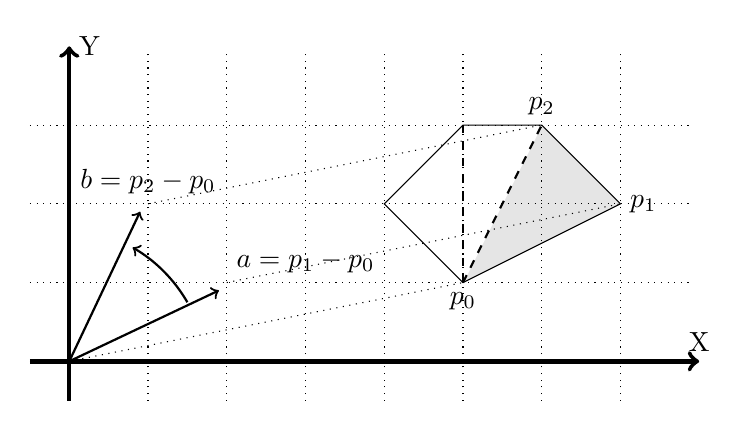
\begin{tikzpicture}
\coordinate (O) at (0,0);
\coordinate (A) at (2,1);
\coordinate (B) at (1,2);
\coordinate (P0) at (5,1);
\coordinate (P1) at (7,2);
\coordinate (P2) at (6,3);
\draw [color=white,fill=gray!20!] (P0) -- (P1) -- (P2) -- cycle;
\draw [] (P0) -- (P1) -- (P2) -- (5,3) -- (4,2) -- cycle;
\draw [step=1cm,dotted] (-0.5,-0.5) grid (7.9,3.9);
\draw [->,ultra thick] (-0.5,0) -- (8,0);
\draw [->,ultra thick] (0,-0.5) -- (0,4);
\node [above] at (8,0) {X};
\node [right] at (0,4) {Y};
\node [above right] at (A) {$a=p_1-p_0$};
\node [above] at (B) {$b=p_2-p_0$};
\draw [->,thick] (O) -- (1.9,0.9);
\draw [->,thick] (O) -- (0.9,1.9);
\draw [->,thick] (1.5,0.75) arc (30:60:1.9);
\draw [thick,dashed] (5,1) -- (6,3);
\draw [thick,dashed] (5,1) -- (5,3);
\node [below] at (P0) {$p_0$};
\node [right] at (P1) {$p_1$};
\node [above] at (P2) {$p_2$};
\draw [dotted] (A) -- (P1);
\draw [dotted] (B) -- (P2);
\draw [dotted] (O) -- (P0);
\end{tikzpicture}
\end{center}

Since a (simple) polygon can be decomposed into triangles, if the area of a triangle can be calculated, the area of a polygon can be calculated. Especially in the case of a convex polygon, it can be neatly divided by triangles formed by one vertex and the edges that do not include that vertex.

\begin{cbox}
xy_t P[110];
int main() {
  // Input example: Let N be the number of points read
  int N=0;
  double x, y;
  while (~scanf("%lf,%lf", &x, &y)) {
    P[N++] = xy_t(x,y);
  }
  // Area calculation
  double sum = 0.0;
  for (int i=0; i+2<N; ++i) {
    xy_t a=P[0], b=P[i+1], c=P[i+2];
    sum += ... // Add the area of triangle abc
  }
  printf("%.10f\n", abs(sum/2.0));
}
\end{cbox}

\begin{tipsbox}{How to read as long as input continues with scanf}
In order to read input lines as long as they can be read, the sample code adopts a loop of \texttt{while (\~{}scanf("\%lf,\%lf", \&x, \&y))}. This is a short (but not very versatile) way and can only be used in an environment where \texttt{\~{}EOF} becomes 0.
\end{tipsbox}

\begin{pybox}
P = [] # Vertex sequence
try:
    while True:
        x,y = map(float,input().split(','))
        P.append(complex(x,y))
except EOFError:
    pass
N = len(P) # Number of vertices
total = 0.0
for i in range(1,N-1):
    a,b,c = P[0],P[i],P[i+1]
    total += cross_product(b-a,c-a) # Add the area of triangle abc
print("{:.10f}".format(abs(total/2.0)))
\end{pybox}

\begin{tipsbox}{How to read as long as input continues with Python3}
If \texttt{input()} is attempted and the input is finished, Python raises an exception called \texttt{EOFError}, so it is surrounded by \texttt{try} in advance and detected by \texttt{except}. When an exception occurs, the \texttt{while} loop where \texttt{input()} was written is exited, and the outer \texttt{except} block is executed (in this case, \texttt{pass}, which does nothing and moves to the next line).
\end{tipsbox}

\begin{psbox}{Polygon - Area}{AOJ}
Calculate the area of a polygon. It is not necessarily convex, but the vertices are given in counterclockwise order.

\aojid{CGL_3_A}

(Similar problem: Area of Polygons (Domestic Preliminary 1998) \aojid{1100} Only the direction in which the vertices are given is different)
\end{psbox}
For a non-convex simple polygon, if the same division as before is performed, triangles will overlap, but if the sum is taken including the sign of the signed area, the correct area can be obtained (surprisingly). The vertices of the polygon must be given in counterclockwise order. Although $p_0$ was used as the center of the division, it is also possible to consider triangles formed by any point (for example, the origin) and each side.

\begin{center}
  \begin{tabular}{ccc}
\begin{tikzpicture}[scale=0.8]
\coordinate (P0) at (2.5,1.5);
\coordinate (P1) at (5,1);
\coordinate (P2) at (3,3);
\coordinate (P3) at (6,3);
\coordinate (P4) at (2,4);
\draw [color=iblue,fill=gray!20!,thick,dashed] (P0) -- (P1) -- (P2) -- cycle;
\draw [] (P0) -- (P1) -- (P2) -- (P3) -- (P4) -- cycle;
\node [below] at (P0) {$p_0$};
\node [right] at (P1) {$p_1$};
\node [above] at (P2) {$p_2$};
\node [right] at (P3) {$p_3$};
\node [left] at (P4) {$p_4$};
\draw [->,ultra thick,dotted,color=iblue] ($(P0)+(1.0,0.6)$) ++(-60:0.5) arc (-60:210:0.5);
\end{tikzpicture}
&
\begin{tikzpicture}[scale=0.8]
\coordinate (P0) at (2.5,1.5);
\coordinate (P1) at (5,1);
\coordinate (P2) at (3,3);
\coordinate (P3) at (6,3);
\coordinate (P4) at (2,4);
\draw [color=iblue,fill=gray!20!,thick,dashed] (P0) -- (P2) -- (P3) -- cycle;
\draw [] (P0) -- (P1) -- (P2) -- (P3) -- (P4) -- cycle;
\node [below] at (P0) {$p_0$};
\node [right] at (P1) {$p_1$};
\node [above] at (P2) {$p_2$};
\node [right] at (P3) {$p_3$};
\node [left] at (P4) {$p_4$};
\draw [->,ultra thick,dotted,color=ired] ($(P0)+(1.6,0.7)$) ++(235:0.5) arc (235:-30:0.5);
\end{tikzpicture}
&
\begin{tikzpicture}[scale=0.8]
\coordinate (P0) at (2.5,1.5);
\coordinate (P1) at (5,1);
\coordinate (P2) at (3,3);
\coordinate (P3) at (6,3);
\coordinate (P4) at (2,4);
\draw [color=iblue,fill=gray!20!,thick,dashed] (P0) -- (P3) -- (P4) -- cycle;
\draw [] (P0) -- (P1) -- (P2) -- (P3) -- (P4) -- cycle;
\node [below] at (P0) {$p_0$};
\node [right] at (P1) {$p_1$};
\node [right] at (P3) {$p_3$};
\node [left] at (P4) {$p_4$};
\draw [->,ultra thick,dotted,color=iblue] ($(P0)+(0.6,1.3)$) ++(-60:0.5) arc (-60:210:0.5);
\end{tikzpicture}
\\
$p_0p_1p_2$ (sgn: +)
&
$p_0p_2p_3$ (sgn: -)
&
$p_0p_3p_4$ (sgn: +)
  \end{tabular}
\end{center}
\subsection{Determining Parallelism}

\begin{psbox}{Parallelism}{PC Koshien 2003}
Overview: Given four distinct coordinate points A = (x1, y1), B = (x2, y2), C = (x3, y3), and D = (x4, y4), determine whether the lines AB and CD are parallel.

The coordinates of the points are given as real numbers with up to 5 decimal places (use this information to estimate numerical errors).

\aojid{0021}
\end{psbox}

Solution Strategy: Determine whether the triangle formed by vectors AB and CD has an area.

\begin{cbox}[emph={eps}]
const double eps = 1e-11;
double x[4], y[4];
int N;
int main() {
    cin >> N; // Number of problems
    for (int t=0; t<N; ++t) {
        for (int i=0; i<4; ++i) 
            cin >> x[i] >> y[i]; // x0,y0..x3,y3
        xy_t a[2] = {
            xy_t(x[0],y[0]) - xy_t(x[1],y[1]), 
            xy_t(x[2],y[2]) - xy_t(x[3],y[3])
        };
        bool p = abs(cross_product(a[0], a[1])) < eps;
        cout << (p ? "YES" : "NO") << endl;
    }
}
\end{cbox}

Note: For determining direction and angle, library functions such as \texttt{sin} and \texttt{arg} can be used, but from the viewpoint of calculation errors, it is better to calculate using the signed area as much as possible. For example, Taylor expansion is used in general implementations of trigonometric functions.
\footnote{Reference: FreeBSD implementation \url{https://svnweb.freebsd.org/base/release/10.1.0/lib/msun/src/k_cos.c?view=markup}}

\begin{pybox}
N = int(input())
for _ in range(N):
    P = list(map(float,input().split()))
    a, b, c, d = [complex(P[i*2],P[i*2+1]) for i in range(4)]
    parallel = abs(cross_product(b-a,d-c)) < 1e-11 # Calculate the boolean value indicating whether ab and cd are parallel
    print("YES" if parallel else "NO")
\end{pybox}

\begin{debugbox}{Operation Check}
  This problem has few sample input/output examples, and the judge data is also not public. Therefore, it is good to try your own test data. For example, long lines, short lines, and the positive/negative sign of the area are examples to check.

For example, the following examples are all ``NO''.
  \begin{terminal}
-0.00001 0 0.00001 0 -0.0001 0 0.00001 0.00001
-100 100 100 100 -100 100 100 99.99999
  \end{terminal}
\end{debugbox}

\medskip

\paragraph{Handling Numerical Errors $\star$}
When using floating-point numbers such as \texttt{double}, numbers that are not represented as the sum of powers of $\frac{1}{2}$ inevitably contain errors (see also Section \ref{section:floating-point-numbers}). In this problem, the input is explicitly stated to have an absolute value of 100 or less, and each value has a maximum of 5 decimal places. Therefore, the effect of errors can be avoided by multiplying by $10^5$ and handling them as integers (\texttt{long long}).
Alternatively, there is a method of predicting the range of errors, such as \texttt{eps} in the sample code.
When errors are added to each element of two vectors $(a,b)$ and $(c,d)$, compare (1) the maximum value of $|ad-bc|$ when they are parallel (0 if there is no error) and (2) the minimum value of $|ad-bc|$ when they are not parallel, and set the threshold so that (1)$<$threshold$<$ (2).
Roughly estimating, (1) is at most
$(4\cdot100)\cdot(100\cdot2^{-54})\approx2.2\cdot10^{-12}$
($100\cdot2^{-54}$ is the representation error when a number up to 100 is represented by \texttt{double}, 400 is
an estimate of the coefficient of $\varepsilon$ when expanding
$|(a+\varepsilon)(d+\varepsilon)-(b+\varepsilon)(c+\varepsilon)|$),
and (2) is about $10^{-10}$ (from the square of the $10^{-5}$ value that can be represented by the input).
Note that, depending on the environment, if you use a relatively new Intel or AMD CPU and a relatively new gcc, you can also perform calculations with better precision of 80-bit or 128-bit by using \texttt{long double} or \texttt{\_\_float128}. There are points to note for each, so please investigate the literature if you use them.
\subsection{Inside/Outside Determination}

\begin{psbox}{A Point in a Triangle}{PC Koshien 2003}
Given a triangle with vertices (x1, y1), (x2, y2), and (x3, y3) on a plane, and a point P(xp, yp), determine whether point P is inside the triangle (excluding the vertices and edges of the triangle).

\aojid{0012}
\end{psbox}
    
Example Solution: Let the vertices of the triangle be a, b, and c. Consider the signed areas of the three triangles pab, pbc, and pca. If p is inside abc, the signs will match; if it is outside, they will not match.

\begin{tabular}{c@{\hspace{3em}}c}
\begin{tikzpicture}[x=2mm,y=2mm]
\fill[ired] (10,10) circle (0.5);
\node[above right] at (10,10) {$p$};
\node[right] at (20,0) {$a$};
\node[above] at (10,20) {$b$};
\node[left] at (0,5) {$c$};
\draw[->, thick] (20,0) edge node [left] {\small Left} (10,20);
\draw[->, thick] (10,20) edge node [right] {\small Left} (0,5);
\draw[->, thick] (0,5) edge node [above] {\small Left} (20,0);
\draw[dotted] (20,0) -- (10,10);
\draw[dotted] (10,20) -- (10,10);
\draw[dotted] (0,5) -- (10,10);
  \begin{scope}[xshift=57,yshift=57,rotate=20]
\draw [->,ultra thick,dotted,color=iblue] (0,0) ++(-30:2.5) arc (-30:90:2.5);
\draw [->,ultra thick,dotted,color=iblue] (0,0) ++(90:2.5) arc (90:210:2.5);
\draw [->,ultra thick,dotted,color=iblue] (0,0) ++(210:2.5) arc (210:330:2.5);
  \end{scope}
\end{tikzpicture}
&
\begin{tikzpicture}[x=2mm,y=2mm]
\fill[ired] (18,15) circle (0.5);
\node[above right] at (18,15) {$p$};
\node[right] at (20,0) {$a$};
\node[above] at (10,20) {$b$};
\node[left] at (0,5) {$c$};
\draw[->] (20,0) edge node [right] {\small Right} (10,20);
\draw[->] (10,20) edge node [right] {\small Left} (0,5);
\draw[->] (0,5) edge node [above] {\small Left} (20,0);
\draw[dotted] (20,0) -- (18,15);
\draw[dotted] (10,20)-- (18,15);
\draw[dotted] (0,5)  -- (18,15);
  \begin{scope}[xshift=57,yshift=57,rotate=20]
\draw [->,ultra thick,dotted,color=ired] (0,0) ++(90:2.5) arc (90:-30:2.5);
\draw [->,ultra thick,dotted,color=iblue] (0,0) ++(90:2.5) arc (90:210:2.5);
\draw [->,ultra thick,dotted,color=iblue] (0,0) ++(210:2.5) arc (210:330:2.5);
  \end{scope}
\end{tikzpicture}\\
Point inside the figure & Point outside the figure
\end{tabular}

\begin{cbox}
double x[4], y[4];
int main() {
    while (true) {
        for (int i=0; i<4; ++i) cin >> x[i] >> y[i];
        if (!cin) break;
        xy_t a(x[0],y[0]), b(x[1],y[1]), c(x[2],y[2]), p(x[3],y[3]);
        // Twice the signed area of pab is \texttt{cross\_product(a-p,b-p)}
        // Twice the signed area of pbc is \texttt{cross\_product(b-p,c-p)}
        // Twice the signed area of pca is \texttt{cross\_product(c-p,a-p)}
        bool ok = signs are the same
        cout << (ok ? "YES" : "NO") << endl;
    }
}
\end{cbox}

For inside/outside determination of polygons that are not necessarily convex, see the next section.
\subsection{Convex Hull}

\begin{pbox}{Convex Polygon - Convex Hull$\star$}{AOJ}
Find the convex hull of a given set of points. Refer to the diagram in the similar problem for what a convex hull is.

(Note: This is a slightly special setting that requires outputting points on the edges.)

\aojid{CGL_4_A}

(Similar problem: Enclose Pins with a Rubber Band (PC Koshien 2004) \aojid{0068} This one has a more straightforward setting)
\end{pbox}

Example Solution: Sort the points by their X-coordinates, and starting from the minimum value (the leftmost point), go right, first constructing the lower half of the outer perimeter.
If, during the process, the direction changes to the right of the current direction of travel (which means that a point that is not originally part of the convex hull has been included), remove all the points that caused this. Perform the same process for the upper half, starting from the rightmost point.

If the number of points is $N$, the above procedure for finding half of the perimeter can be done in $O(N)$, so the total computation time, including the time required for sorting, is $O(N\log N)$.

\begin{center}
\begin{tabular}{c@{\hspace{3em}}c@{\hspace{3em}}c}
\begin{tikzpicture}[scale=0.8]
\coordinate (P0) at (2,4);
\coordinate (P1) at (2.5,1.5);
\coordinate (P2) at (3,3);
\coordinate (P3) at (5,1);
\coordinate (P4) at (6,3);
\draw [] (P0) circle (2.5pt);
\draw [] (P1) circle (2.5pt);
\draw [] (P2) circle (2.5pt);
\draw [] (P3) circle (2.5pt);
\draw [] (P4) circle (2.5pt);
\draw (P0) -- (P1);
\end{tikzpicture}
&
\begin{tikzpicture}[scale=0.8]
\coordinate (P0) at (2,4);
\coordinate (P1) at (2.5,1.5);
\coordinate (P2) at (3,3);
\coordinate (P3) at (5,1);
\coordinate (P4) at (6,3);
\draw [] (P0) circle (2.5pt);
\draw [] (P1) circle (2.5pt);
\draw [] (P2) circle (2.5pt);
\draw [] (P3) circle (2.5pt);
\draw [] (P4) circle (2.5pt);
\draw (P0) -- (P1) -- (P2);
\end{tikzpicture}
&
\begin{tikzpicture}[scale=0.8]
\coordinate (P0) at (2,4);
\coordinate (P1) at (2.5,1.5);
\coordinate (P2) at (3,3);
\coordinate (P3) at (5,1);
\coordinate (P4) at (6,3);
\draw [] (P0) circle (2.5pt);
\draw [] (P1) circle (2.5pt);
\draw [] (P2) circle (2.5pt);
\draw [] (P3) circle (2.5pt);
\draw [] (P4) circle (2.5pt);
\draw (P0) -- (P1) -- (P2);
\draw[thick,dashed] (P2) -- (P3);
\end{tikzpicture}
\\
t=0: From the leftmost (minimum x-coordinate)
&
t=1: Connect the lines in order
&
t=2: If it turns right
\\
\begin{tikzpicture}[scale=0.8]
\coordinate (P0) at (2,4);
\coordinate (P1) at (2.5,1.5);
\coordinate (P2) at (3,3);
\coordinate (P3) at (5,1);
\coordinate (P4) at (6,3);
\draw [] (P0) circle (2.5pt);
\draw [] (P1) circle (2.5pt);
\draw [] (P2) circle (2.5pt);
\draw [] (P3) circle (2.5pt);
\draw [] (P4) circle (2.5pt);
\draw (P0) -- (P1) -- (P3);
\end{tikzpicture}
&
\begin{tikzpicture}[scale=0.8]
\coordinate (P0) at (2,4);
\coordinate (P1) at (2.5,1.5);
\coordinate (P2) at (3,3);
\coordinate (P3) at (5,1);
\coordinate (P4) at (6,3);
\draw [] (P0) circle (2.5pt);
\draw [] (P1) circle (2.5pt);
\draw [] (P2) circle (2.5pt);
\draw [] (P3) circle (2.5pt);
\draw [] (P4) circle (2.5pt);
\draw (P0) -- (P1) -- (P3) -- (P4);
\end{tikzpicture}
\\
t=4: Delete unnecessary points and reconnect
&
t=5: Lower side complete
\end{tabular}
\end{center}

\paragraph{Sorting Points}

Since the C++ complex number type (complex) does not have comparison operators defined, it is necessary to define them yourself. If you define \texttt{operator<} in the \texttt{std} namespace as in the example below, it will be automatically used by \texttt{sort}.
As a comparison criterion, use something such that \texttt{a==b} if \texttt{!(a<b)} and \texttt{!(b<a)} are both true.\footnote{\url{https://en.cppreference.com/w/cpp/named_req/Compare}}

\begin{cbox}[emph={std}]
namespace std {
  bool operator<(xy_t l, xy_t r) {
    return (l.real()!=r.real()) ? l.real()<r.real() : l.imag()<r.imag();
  }
  // Alternative: When aligning with std::pair
  bool operator<(xy_t l, xy_t r) {
    return make_pair(l.real(), l.imag()) < make_pair(r.real(), r.imag());
  }
}
  
\end{cbox}
\section{Various Topics}

\begin{psbox}{A Symmetric Point}{PC Koshien 2005}
Output the point that is symmetrical to point Q with respect to a line.

\aojid{0081}
\end{psbox}

Example Solution: Let S be the point where Q is projected onto the line. Then, the desired point R is at the position where S is translated by the vector QS. For processing comma-separated input and controlling the number of decimal places in the output, it is convenient to use \texttt{scanf} and \texttt{printf} after \texttt{\#include<cstdio>} as follows.

\begin{cbox}
#include <cstdio>
double X1,Y1,X2,Y2,XQ,YQ;
  
int main() {
  while (~scanf("%lf,%lf,%lf,%lf,%lf,%lf",
                 &X1, &Y1, &X2, &Y2, &XQ, &YQ)) {
    xy_t P1(X1,Y1), P2(X2,Y2), Q(XQ,YQ);
    xy_t R = ...; // Calculate the point of line symmetry
    printf("%.10f,%.10f\n", R.real(), R.imag());
  }
}
\end{cbox}

\begin{pbox}{Polygon - Polygon-Point Containment}{AOJ}
Determine whether a point is inside or outside a polygon that is not necessarily convex.

\aojid{CGL_3_C}
\end{pbox}
(Note: Normally, it is difficult to determine whether a point is on an edge, but it is possible in this case because the coordinates are integers.)

Example Solution: Extend a half-line from the point you want to check in any direction and count the number of edges it crosses. If it is even, it is outside; if it is odd, it is inside. It is necessary to prepare functions in advance, such as whether a line segment has an intersection with a line. If the half-line passes very close to a vertex, it is safer to change the angle to avoid worrying about the effects of errors.

\begin{pbox}{Point Set - Closest Pair$\star$}{AOJ}
Find the closest pair of points.

\aojid{CGL_5_A}
\end{pbox}

If the number of points is $N$, trying all pairs of points requires $O(N^2)$ time, but it is possible in $O(N\log N)$ using divide and conquer. There also exists a randomized algorithm with $O(N)$.

Divide and Conquer Strategy: Sort the points by X-coordinate and Y-coordinate, respectively. Divide the points in half by the X-coordinate, and recursively find the closest pair in the left and right halves. Let $d$ be the smaller of the two minimum distances found. The closest pair of the whole is either the closest pair of the left half, the closest pair of the right half, or the closest pair of a point in the left half and a point in the right half. For the latter, when the points within a distance $d$ from the dividing line between the left and right halves are sorted by Y-coordinate, it can be determined in a linear number of calculation steps with respect to the number of points by using the property that only pairs within a constant number (e.g., 8) are candidates. The proof is based on the fact that points cannot exist too densely with the restriction of $d$ when considering an appropriate square grid around the dividing line. In the implementation, it is not possible to achieve $O(N\log N)$ if the points are sorted by Y-coordinate every time. It is better to sort the whole set once at the beginning and then distribute them during the division. Also, when dividing, it may be necessary to pay attention to the case where multiple points have the same Y-coordinate. In practice, this can be avoided by rotating the whole set randomly at the beginning.
\section{Applied Problems}

\begin{pbox}{ConvexCut}{Summer Camp 2012}
Determine if there exists a point in a given figure such that it can be cut into two equal areas regardless of the cutting angle.

\aojid{2442}
\end{pbox}

It can be proven that this is only possible when the polygon has an even number of vertices and all pairs of edges that should be paired are parallel, or when the midpoints of the paired vertices are equal.

Example Answer (Input/Output)
\begin{cbox}
#include <complex>
#include <iostream>
#include <cstdio>
using namespace std;
int N, x, y;
typedef complex<double> xy_t;
xy_t P[60];
void solve() {
 ...
}
int main() {
    while (cin >> N) {
        for (int i=0; i<N; ++i) {
            cin >> x >> y;
            P[i] = xy_t(x,y);
        }
        solve();
    }
} 
\end{cbox}

Example Answer (Midpoint Calculation)
\begin{cbox}
void solve() {
  // If it's odd, there is no such point
  ...
  xy_t a = (P[0]+P[N/2])*0.5; // Midpoint of P[0] and P[N/2]
  for (int i=1; i<N/2; ++i) {
    xy_t b = ... // Midpoint of P[i] and P[i+N/2]
    // If a and b do not match even with error considered, abs(a-b) > eps, there is no such point
  }
  printf("YES\n");
}  
\end{cbox}

\begin{pbox}{Circle and Points$\star$}{National Preliminary 2004}
N points are given on the xy-plane. Move a circle of radius 1 on the xy-plane to enclose as many of these points as possible. At this time, answer the maximum number of points that can be enclosed simultaneously. Here, a circle "encloses" a point if the point is inside or on the circumference of the circle. (This problem statement has sufficient descriptions regarding errors)

\aojid{1132}
\end{pbox}

Since there are an infinite number of candidate circle positions, narrow down the candidates.
("Consider the limit" \pccbook[p.~229])

\begin{tipsbox}{Way of Thinking}
Let n be the maximum number of points that can be enclosed simultaneously, and assume there is a circle that encloses n points. If no point is touching the circle, even if you move it until one of the points inside touches, the number of points enclosed will not change.
That is, it is sufficient to consider only circles that touch one of the points (even if you consider the remaining circles, the answer will not change). However, there are still an infinite number of such circles.

Assume there is a circle that encloses n points, and one point is on the circle. If you rotate the circle around that point \textcolor{white}{as the center, the number of points enclosed will not change until a new point inside touches the circle.
That is, it is sufficient to consider only circles that pass through two points (even if you consider the remaining circles, the answer will not change). There are only about $2N^2$ such circles.}
\end{tipsbox}

\begin{debugbox}{Caution for Exceptional Cases}
The above idea is generally correct, but there are exceptional cases. That is, \textcolor{white}{when the answer is 1, the circle that gives the maximum does not have} the above property.
\end{debugbox}

\begin{debugbox}{How to Count Points}
  Suppose you want to set the position of a circle that exactly covers a certain point p and check the number of points included in it. For that purpose, if you calculate the distance to the center of the circle for all points, you can generally determine it. However, for the point p itself, since it is located on the circle, it may be determined to be outside due to numerical errors. If you increase the tolerance here, there is a risk of determining points that are truly outside as inside. Therefore, the determination of point p should be treated specially, and \textcolor{white}{it is better to use the identity of the id (what number it is if the points are managed in an array) without calculating the distance.}
\end{debugbox}

Example Answer:

\begin{cbox}
int main() {
  // Initialize the maximum value
  for (/*point p*/) {
    for (/*point q*/) { // p!=q
      if (/*if there is a circle passing through pq*/) { // There can be 0, 1, or 2 cases
         /*Count the number of points inside while checking all points*/
         /*Update if it exceeds the maximum value*/
      }
    }
  }
}
\end{cbox}


\begin{pbox}{Roll-A-Big-Ball}{National Preliminary 2008}
Find the maximum size of a large ball that satisfies the conditions.

  \aojid{1157}
\end{pbox}

\begin{pbox}{Space Golf}{Asian Tournament 2014}
  
  \aojid{1348}
\end{pbox}

\begin{pbox}{Chain-Confined Path$\star$}{National Preliminary 2012}
  Find the shortest path through a ring.

\aojid{1183}
\end{pbox}

Hint: Consider the shape of the shortest path.
 
Solution: \textcolor{white}{Let the start point, end point, and the intersection points of each circle be vertices, find if it is possible to move in a straight line between each point to create edges, and solve the shortest path problem.}

\begin{pbox}{Neko's Treasure$\star$}{Mock Regional Preliminary 2009}
Find how many walls to overcome (refer to the problem statement).

\aojid{2181}
\end{pbox}

\begin{pbox}{Area of Polygons$\star$}{Asian Tournament 2003}
Find the area of the shaded part.

\aojid{1242}
\end{pbox}
Way of thinking: It's just a matter of slicing and summing, but there are quite a few points to note, such as when multiple lines pass through the same square.

Reference: \url{http://www.ipsj.or.jp/07editj/promenade/4501.pdf}

\begin{pbox}{Treasure Hunt$\star$}{Summer Camp 2012}
Count the treasures in the area (efficiently).

\aojid{2426}
\end{pbox}

If you count naively, it will take too much time, so perform preprocessing when the points are given and prepare to answer the questions.
As a data structure for efficiently answering questions, for example, a quad tree can be used.



\begin{pbox}{Altars$\star\star$}{6th Polish Olympiad in Informatics}
A pillow that says that in China, evil spirits are believed to travel in straight lines.

There is a rectangular temple with an altar in the center. The walls of the temple are either east-west or north-south. The entrance to the temple is in the middle of one side. Check if there is a line of sight from the outside to the altar.

\url{http://main.edu.pl/en/archive/oi/6/olt}  
\end{pbox}

\begin{pbox}{Fish$\star\star$}{Algorithmic Engagements 2009}
There are fish that wake up/go to sleep at the same time every day. When they wake up, they may be shifted by one square due to ocean currents. They swim so that they can see their position at the same time yesterday. They can accelerate and decelerate freely. There are many records of the fish's movements for one day, but the dates are unknown. What is the minimum number of fish that can be said to be observed?

\url{http://main.edu.pl/en/archive/pa/2009/ryb}  
\end{pbox}
 \chapter{Simple Parsing}\label{chapter:parsing}

\begin{itembox}[l]{Example Problems}
Let's make a computer understand a string written in a specific grammar:
  \begin{itemize}
\setlength{\itemsep}{0pt}
  \item $( V | V ) \& F \& ( F| V)$ \dingright $F$ (Boolean calculation)
  \item 35=1?((2*(3*4))+(5+6)) \dingright '+'  (Operator estimation)
  \item 4*x+2=19 \dingright x=4.25 (Solving equations)
  \item C2H5OH+3O2+3(SiO2) == 2CO2+3H2O+3SiO2 (Calculation of molecular weight)
  \end{itemize}  
\end{itembox}

\section{Creating Arithmetic Operations}
\subsection{Let's Try Making Addition}

\paragraph{Global Variables}:
\begin{cbox}
const string S = "12+3";
size_t cur = 0; // Abbreviation for cursor, the parsing start position
int parse();
\end{cbox}

Execution Example: (We will create something that works as follows)
\begin{cbox}
int main() {
  int a = parse();
  assert(a == 15);
  assert(cur == S.size());
}  
\end{cbox}

\begin{pybox}
S = "0"
cur = 0

a = parse()
assert a == 15
assert cur == len(S)
\end{pybox}

\paragraph{Preparing a Function to Read One Character}

\begin{cbox}[emph={readchar,peek}]
// Reads one character and advances cur
char readchar() { 
  assert(cur < S.size());    
  char ret = S[cur];
  cur += 1;
  return ret;
  // It can also be written in one line as return S[cur++];
}
// Reads one character but does not advance cur
char peek() { 
  assert(cur < S.size());    
  return S[cur];
}
\end{cbox}

In Python, to change a global variable within a function, specify it with \tindex{global}.
\begin{pybox}[emph=global]
def readchar():
    global cur
    c = S[cur]
    cur += 1
    return c
def peek():
    return S[cur]
\end{pybox}

\paragraph{What is assert?} 
(Re-posted)
\begin{cbox}[emph={cassert,assert}]
#include <cassert>
int factorial(int n) {
  assert(n > 0); // (*)
  if (n == 1) return 1;
  return n * factorial(n-1);
}     
\end{cbox}

Execution Example
\begin{cbox}
cout << factorial(3) << endl; // Displays 6
cout << factorial(-3) << endl; // Stops by displaying the line number of (*)
\end{cbox}

\subsubsection{First Addition}

\begin{itembox}[l]{(Rough) Grammar of Addition}
  \begin{alltt}
Expression := Number '+' Number
Number := Repetition of Digit
Digit := '0' | '1' | ... | '9'\end{alltt}  
\end{itembox}

How to read: (Reference: (Extended) BNF)
\begin{itemize}
\setlength{\itemsep}{0pt}
\item \texttt{P := Q} \dingright Definition of a grammar rule named P
\item \texttt{A B} \dingright B follows A
\item \texttt{'a'} \dingright Character a
\item \texttt{x | y} \dingright x or y
\end{itemize}


\subsubsection{Implementing According to the Grammar (Digit)}
\texttt{\textcolor{ired}{Digit := '0' | '1' | ... | '9'}}

\begin{cbox}[emph={digit,peek,readchar}]
#include <cctype>
int digit() {
  assert(isdigit(peek()));  // Check that S[cur] is a digit
  int n = readchar() - '0'; // Convert '0' to 0
  return n;
}
\end{cbox}
Conversion of characters to numbers: In C and C++, characters are managed by numbers representing those characters. Although the character code is not specified in the language standard, it can be considered as the \eindex{ASCII} code in the environment we currently use. In it, using the fact that characters such as '0', '1', '2', ..., 'a', 'b', 'c' are assigned codes in order, the above subtraction shows how many characters after '0' it is, which is the numerical value we want. One way to check the ASCII code table is to use the man command, which is convenient. You can type \texttt{man ascii} in the terminal.

\begin{pybox}
def digit():
  assert peek().isdigit()
  n = int(readchar()) # Read one character and convert it to a number
  return n;
\end{pybox}

In the case of Python, it is good to determine with \texttt{isdigit()} as above and convert with \texttt{int}.

\subsubsection{Implementing According to the Grammar (Number)}
\texttt{\textcolor{ired}{Number := Repetition of Digit}}

\begin{cbox}[emph={number},emph={[2]digit}]
int number() {
  int n = digit();
  while (cur < S.size() && isdigit(peek())) // Look ahead one character to see if the next is also a digit
    n = n*10 + digit(); 
  return n;
}
\end{cbox}

\begin{pybox}[emph={number},emph={[2]digit}]
def number():
    n = digit()
    while cur < len(S) and peek().isdigit():
        n = n*10+digit()
    return n  
\end{pybox}

\subsubsection{Implementing According to the Grammar (Expression)}
\texttt{\textcolor{ired}{Expression := Number '+' Number}}

\begin{cbox}[emph={expression},emph={[2]number}]
int expression() {
  int a = number();
  char op = readchar();
  int b = number();
  assert(op == '+');
  return a + b;
}
\end{cbox}

This should work if it's just addition:
\begin{cbox}
const string S = "12+3";
size_t cur = 0; // Parsing start position
.. 
int parse() { return expression(); }
int main() {
  int a = parse();
  cout << a << endl; // 15 should be output;
}  
\end{cbox}

\paragraph{Test}
Try not only ``12+5'' but also ``1023+888'', etc.

\subsubsection{Extension: Add Subtraction}
Let's try ``12-5'' instead of ``12+5''

Method: Determine if op is '+' or '-' in the expression function
\begin{cbox}
  if (op == '+') return a + b;
  else return a - b;  
\end{cbox}
(Also rewrite assert appropriately)

\subsubsection{Extension: Add Three or More}
Let's try ``1+2+3+4'' instead of ``12+5''

Rewrite expression to allow multiple additions
\begin{cbox}[emph={sum,while}]
int expression() {
    int sum = number();
    while (cur < S.size() && (peek() == '+' || peek() == '-')) {
        // While addition or subtraction continues
        char op = readchar();
        int b = number();
        if (op == '+') add b to sum;
        else subtract b from sum;
    }
    return sum;
}
\end{cbox}


\subsubsection{Next Extensions}
  \begin{itemize}
\setlength{\itemsep}{0pt}
  \item Support multiplication and division: \\
    Create new rules because the precedence of operators changes
  \item Support (multiple) parentheses: \\
    Create new rules and recurse
  \end{itemize}
\subsection{Arithmetic Operations Without Parentheses (Rough) Grammar}

\begin{itembox}[l]{(Rough) Grammar of Arithmetic Operations}
  \begin{alltt}
Expression := Term \{ ('+'|'-') Term \}
Term := Number \{ ('*'|'/') Number \}
Number := Digit \{ Digit \}
\end{alltt}
\end{itembox}

How to read: (Reference: (Extended) BNF)
\begin{itemize}
\setlength{\itemsep}{0pt}
\item \texttt{A B} \dingright B follows A
\item \texttt{\{C\}} \dingright Zero or more repetitions of C
\end{itemize}

Example: 5*3-8/4-9
\begin{itemize}
\setlength{\itemsep}{0pt}
\item Term: 5*3, 8/4, 9
\item Number: 5, 3, 8, 4, 9
\end{itemize}

\subsubsection{Implementation of Arithmetic Operations (Term)}
\texttt{\textcolor{ired}{Term := Number \{ ('*'|'/') Number \}}}

  \begin{cbox}[emph={term},emph={[2]number,*,/}]
int term() {
  int a = number();
  while (cur < S.size() 
        && (peek() == '*' || peek() == '/')) {
    char op = readchar();
    int b = number();
    if (op == '*') a *= b; else a /= b;
  }
  return a;
}
\end{cbox}

In Python, integer division is possible with the \texttt{//} operator, but it is slightly different from the specifications of this problem. That is, in this problem, it seems necessary to evaluate \texttt{3/-2} as -1 instead of -2. Therefore, we use the \texttt{math.\tindex{trunc}} function.
\begin{pybox}[emph={term},emph={[2]number,*,/}]
import math
def term():
    a = number()
    while cur < len(S) and (peek() == '*' or peek() == '/'):
        op = readchar()
        b = number()
        a = a*b if op == '*' else math.trunc(a/b)
    return a
\end{pybox}
  
\subsubsection{Implementation of Arithmetic Operations (Expression)}
\texttt{\textcolor{ired}{Expression := Term \{ ('+'|'-') Term \}}}

  \begin{cbox}[emph={expression},emph={[2]term,+,-}]
int expression() {
  int a = term();
  while (cur < S.size())
      && (peek() == '+' || peek() == '-')) {
    char op = readchar();
    int b = term();
    if (op == '+') a += b; else a -= b;
  }
  return a;
}
\end{cbox}
\subsection{Arithmetic Operations: Introducing Parentheses}
The entire expression, represented by Expression, appears again inside parentheses \dingright Process recursively

\begin{itembox}[l]{Grammar with Parentheses Introduced}
  \begin{alltt}
Expression := Term \{ ('+'|'-') Term \}
Term := \textcolor{ired}{Factor} \{ ('*'|'/') \textcolor{red}{Factor} \}
\textcolor{ired}{Factor := '(' Expression ')' | Number}
\end{alltt}
\end{itembox}

An example implementation of \texttt{factor()} is as follows:
  \begin{cbox}[emph={factor},emph={[2]number,expression}]
int expression(); // Forward declaration
int factor() {
  if (peek() != '(') return number();
  readchar(); // Discard '('
  int n = expression();
  assert(peek() == ')');
  readchar(); // Discard ')'
  return n;
}
\end{cbox}

The implementation of \texttt{term()} should also be adjusted to match the grammar.

\subsection{Summary}
Summary of implementation:
  \begin{itemize}
\setlength{\itemsep}{0pt}
  \item Create functions corresponding to the grammar rules
  \item The return value type should be what you want after parsing is complete
    \begin{itemize}
\setlength{\itemsep}{0pt}
    \item Arithmetic operations \dingright Integer
    \item Polynomial \dingright Coefficients of each degree
    \item Molecular formula \dingright Molecular weight, number of each atom...
    \end{itemize}
  \end{itemize}

Grammar description:
  \begin{itemize}
\setlength{\itemsep}{0pt}
  \item Points to note: Operator precedence, left-associativity, and right-associativity
  \item Restriction: Be able to determine the appropriate rule with one character lookahead (LL(1))
  \end{itemize}


\paragraph{Supplement}

Should the repetition of \texttt{P := A \{ '+' A \}} be described recursively?
\begin{itemize}
\setlength{\itemsep}{0pt}
\item \texttt{P := P '+' A | A}\\
\dingright If implemented as is, P will recurse indefinitely
\item If converted to right-associativity, parsing is possible
  \begin{itemize}
\setlength{\itemsep}{0pt}
  \item \texttt{P := A P'}
  \item \texttt{P' := '+' A P' | $\epsilon$}
  \end{itemize}
($\epsilon$ is the empty string)
\end{itemize}

\section{Practice Problems}

\begin{pbox}{Smart Calculator}{PC Koshien 2005}
Create a calculator.

  \aojid{0109}
\end{pbox}

Example Solution:
\begin{cbox}
/*const*/ string S; // Removed const attribute because the value is changed
...
int main() {
    int N;
    cin >> N;
    for (int i=0; i<N; ++i) {
        cur = 0;
        cin >> S;
        S.resize(S.size()-1); // Ignore the last =
        cout << expression() << endl;
    }
}  
\end{cbox}

\begin{pbox}{Molecular Formula}{Asian Regional 2003}
Based on the atomic weights of each atom, find the molecular weight of each molecule.

\aojid{1244}
\end{pbox}

If you create a table at the beginning so that atoms can be converted to atomic weights, the rest is just multiplication and addition operations.

\begin{pbox}{How Can I Satisfy You? Let's Count Them Up}{National Preliminary 2008}
Find the assignments of variables that satisfy a logical expression.

\aojid{1155}
\end{pbox}

Example Solution:
\begin{enumerate}
\item If there are no variables, it is easy to find the value of the expression. That is, it is sufficient to replace P, Q, and R inside the string with 0, 1, and 2, respectively, and then parse and calculate. Since there are $3^3$ ways to assign values to P, Q, and R, repeat that many times.
\item (Especially recommended in C++11) Assume that the assignment of values to P, Q, and R is represented by an integer array \texttt{int a[3]}. Create a function by parsing that takes the assignment \texttt{a} as an argument and returns the value of the expression with that assignment. The part that utilizes the parsing result is as follows:
  \begin{c11box}
int solve() {
    cur = 0;
    auto tree = parse();
    int count = 0;
    for (int p:{0,1,2})
	for (int q:{0,1,2})
	    for (int r:{0,1,2}) {
		int a[] = {p, q, r};
		if (tree(a) == 2) ++count;
	    }
    return count;
}    
  \end{c11box}
The function that returns the value of the expression for an assignment is created by combining detailed functions. For example, if the character \texttt{c} represents a number, create a constant function that returns the same value regardless of the assignment: \texttt{return [=](int[3])\{ return c-'0'; \};}. If it is an alphabet, it returns a value according to the argument, so it should be \texttt{return [=](int a[3])\{
  return a[c-'P']; \};}. In the case of a binary operator enclosed in parentheses, after creating functions such as \texttt{left} and \texttt{right} that analyze the left and right sides in the same way as in the four arithmetic operations, create a function that calls the left and right functions like \texttt{return [=](int a[3]) \{ return min(left(a), right(a)); \};}.
\begin{c11box}
#include <functional>
typedef function<int(int[3])> node_t;
node_t parse() {
    char c = S[cur++];
    if (isdigit(c))
	return [=](int[3]){ return c-'0'; };
    if (isalpha(c))
	return [=](int a[3]){ return a[c-'P']; };
    node_t left = parse();
    if (c == '-')  // Perform the '-' operation on \texttt{left(a)}
	return [=](int a[3]) { return ...; };
    assert(c == '(');
    char op = S[cur++];
    node_t right = parse();
    ++cur; // ')'
    // Since the following is a binary operator, for \texttt{left(a)} and \texttt{right(a)}...
    if (op == '*')
	return [=](int a[3]) { return ...; }; // Perform the '*' operation
    return [=](int a[3]) { return ...; }; // Perform the same '+' operation
}  
\end{c11box}
\end{enumerate}

\begin{pbox}{Equation Solver}{Ulm Local 1997}
Solve a simple equation.

\url{http://poj.org/problem?id=2252}
\end{pbox}

Example Solution: Parse the right and left sides respectively, and compare the coefficients of the first order and the constant terms on both sides.

\begin{pbox}{Matrix Calculator}{Asian Regional 2010}
Let's do matrix multiplication.

\aojid{1314}
\end{pbox}

\begin{pbox}{ASCII Expression}{Asian Regional 2011}
Calculate arithmetic expressions drawn in ASCII art style.

  \aojid{1322}
\end{pbox}

\begin{pbox}{Chemist's Math}{Asian Regional 2009}
Find the ratio of each substance required for a given reaction.
  
\aojid{1300}
\end{pbox}
Example Solution: Investigate the composition of each molecule and solve the system of equations.

\begin{pbox}{Questions$\star\star$}{Algorithmic Engagements 2008}

Skillfully simulate the knowledge states of P princes and wizards, and guess how they would answer questions.

\url{http://main.edu.pl/en/archive/pa/2008/pyt}
\end{pbox}

Supplement
\begin{itemize}
\setlength{\itemsep}{0pt}
\item Limitations: It is written that the maximum number of possible variable combinations is 600, and the absolute value of the variable values during calculation does not exceed 1 million, which are important points.
\item In the sample input and explanation, it says ``S 1 7 All sons know that there are less than 3 golden
  crowns.'', but since there is ``M 1 7'' immediately after, this explanation is correct. Otherwise, the actual value of variable 7 cannot be read from ``S 1 7''.
\item The person in charge's answer is about 160 lines.
\end{itemize}
 \chapter{Repeated Squaring and Matrix Exponentiation}\label{chapter:rsquares}

\begin{itembox}[l]{Overview}
Experience how computation time can be shortened by using appropriate methods.
In problems where this method is applicable, it is also possible to easily find the simulation result after 1 billion steps.

Applications:
    \begin{itemize}
\setlength{\itemsep}{0pt}
    \item Find all the places you can go when a dice roll of $N (0\le N\le {2^{31}})$ occurs in a sugoroku game.
    \item Find the state of a biological colony that reproduces according to rules after N turns.
    \item Find the number of ways to paint according to rules.
    \end{itemize}
(\pccbook[p.~114])
\end{itembox}
\section{Approach}

Let's consider the calculation of $3^8 = 6561$ as an example.
\begin{itemize}
\setlength{\itemsep}{0pt}
\item $3\cdot{}3\cdot{}3\cdot{}3\cdot{}3\cdot{}3\cdot{}3\cdot{}3$ \dingright{} 7 multiplications
\item \texttt{int a = 3*3, b = a*a, c = b*b;} \dingright{} 3 multiplications
\end{itemize}

Exercise: What about $3^{128}$? \dingright{} $\log(128)$ multiplications

\begin{psbox}{Elementary Number Theory - Power}{AOJ}
For two integers $m$ and $n$, find the remainder of $m^n$ when divided by $1\,000\,000\,007$.

  \aojid{NTL_1_B}
\end{psbox}

Related:
\begin{itemize}
\setlength{\itemsep}{0pt}
\item Be careful of overflow: The range that can be represented by int is about 2 billion in this environment.
\item Handling of remainders: (a*b)\%M = ((a\%M)*(b\%M))\%M
\end{itemize}
See \pcaojbook[pp.~445--].

\section{Language Features: struct and Recursive Functions}
In this chapter, we will use \texttt{long long} and \texttt{struct}.
Refer to Appendix \ref{section:long-long} and \ref{section:struct} as needed.

\section{Representation and Operations of Square Matrices}
Note: The following is a sample code for a 2x2 matrix. You can create an NxN matrix yourself by using data structures such as arrays, vectors, or valarrays. If you need it for research or work, it is safer to use a dedicated library.

\begin{cbox}
struct Matrix2x2 {
  int a, b, c, d; // a,b are the upper row, c,d are the lower row
};
\end{cbox}

Let's also create a display function.

\begin{cbox}
void show(Matrix2x2 A) { 
    cout << "[ " << endl
         << A.a << ' ' << A.b << endl
         << A.c << ' ' << A.d << endl
         << "]" << endl;
}
\end{cbox}

\paragraph{Multiplication of Matrices}
Next, we define multiplication. The following \texttt{mult} calculates the product of matrices \texttt{A, B}.

\begin{cbox}  
// returns C = A*B
Matrix2x2 mult(Matrix2x2 A, Matrix2x2 B) {
    Matrix2x2 C = {0}; // Initialize with 0
    C.a = A.a * B.a + A.b * B.c;
    C.b = A.a * B.b + A.b * B.d;
    C.c = A.c * B.a + A.d * B.c;
    C.d = A.c * B.b + A.d * B.d;
    return C;
}
// (Note) Be careful as exponentiation calculations can easily overflow: It is often necessary to add some tricks here.
\end{cbox}

Example of use:

\begin{cbox}
  Matrix2x2 A = {0,1, 2,3}, B = {0, 1, 2, 0};
  show(A);
  show(B);
  Matrix2x2 C = mult(A, B);
  show(C);
\end{cbox}

\paragraph{Calculation of Exponentiation (Repeated Squaring)}

The following code calculates $A^p$ (where $p>0$) of matrix A and writes it to O.

\begin{cbox}
// O = \(A\sp{p}\) 
Matrix2x2 expt(Matrix2x2 A, int p) {
    if (p == 1) {
        return A;
    } else if (p % 2 == 1) {
        Matrix2x2 T = expt(A, p-1);
        return mult(A, T); 
    } else {
        Matrix2x2 T = expt(A, p/2);
        return mult(T, T);  
    }
}
\end{cbox}

Example of use:

\begin{cbox}
  Matrix2x2 A = {0,1, 2,3};
  Matrix2x2 C = expt(A, 3); // A to the power of 3
  show(C);
\end{cbox}

\section{Practice: Fibonacci Numbers}

\begin{pbox}{Fibonacci}{Stanford Local 2006}
Calculate the remainder when the n-th value of the Fibonacci sequence is divided by $10^4$.

$0\le n \le 10^{16}$

\url{http://poj.org/problem?id=3070}
\end{pbox}

\subsection{Various Calculation Strategies}\label{section:fibonacci}

\subsubsection*{Strategy 1: Calculate According to the Definition}

\begin{cbox}
int fib(int n) {
    if (n == 0) return 0;
    if (n == 1) return 1;
    return fib(n-2)+fib(n-1);
}
\end{cbox}

Example of use:

\begin{cbox}
int main() {
  for (int i=1; i<1000; ++i)
    cout << "fib" << i << " = " << fib(i) << '\n';
}
\end{cbox}

Around n = 30, it stops progressing.

\subsubsection*{Strategy 2: Memorize Calculations Once Performed}\label{section:memoization}

Let's prepare an array called table and memorize the calculations once performed. This technique is called \eindex{memoization} (\eindex{tabling}) and has a wide range of applications.

\begin{cbox}
int table[2000]; // Memorize answers up to 2000
int fibmemo(int n) {
    if (n == 0) return 0;
    if (n == 1) return 1;
    if (table[n] == 0) // If it's the first time
      table[n] = fibmemo(n-2)+fibmemo(n-1); // Calculate and memorize
    return table[n]; // Return the memorized value
}
\end{cbox}

Now, even for n=1000, the answer can be obtained immediately. (Although it overflows, we will ignore it for now)

However, with this method, it is only possible to calculate up to the number of elements in the \texttt{table} array. In the problem, the maximum value of n is $10^{16}$, so it is not realistic.

\subsubsection*{Strategy 3: Calculate from the Smallest}
It can be calculated in time proportional to $n$. With this method, if you wait, it will finish around $10^{9}$, but $10^{16}$ takes too long.

\begin{cbox}
int fibl(int n) {
    int a[2] = {0,1};
    for (int i=2; i<=n; ++i) {
        // Invariant: At the start of the loop, a[0] and a[1] are respectively
        //   Fib(i-1) and Fib(i-2) (if i is odd)
        //   Fib(i-2) and Fib(i-1) (if i is even)
        a[i%2] = a[0] + a[1];
    }
    return a[n%2];
}
\end{cbox}
\subsection{Representation with Matrices}

$$\left(
\begin{array}{cc}
  F_{n+2} \\ F_{n+1}
\end{array}\right)
 = 
\left(\begin{array}{cc}
  1 \phantom{x} 1 \\ 1 \phantom{x} 0
\end{array}\right)
\left(\begin{array}{cc}
  F_{n+1} \\ F_n
\end{array}\right)
$$

If we let $A = \left(\begin{array}{cc}
  1 \phantom{x} 1 \\ 1 \phantom{x} 0
\end{array}\right)$, then from the associative property, we obtain:
$$\left(
\begin{array}{cc}
  F_{n+1} \\ F_{n}
\end{array}\right)
 = A^n
\left(\begin{array}{cc}
  F_{1} \\ F_0
\end{array}\right)
 = A^n
\left(\begin{array}{cc}
  1 \\ 0
\end{array}\right).
$$

With this approach, even if $n$ becomes as large as $10^{16}$, it can be calculated realistically. However, since $n$ exceeds the range that can be represented by \texttt{int}, use \texttt{long long} for the arguments of \texttt{expt()}, etc.
Also, if calculated normally, the values of the elements will also exceed the range that can be represented by \texttt{int}, so use properties such as:
\begin{itemize}
\item (a*b)\%M = ((a\%M)*(b\%M))\%M
\item (a+b)\%M = ((a\%M)+(b\%M))\%M
\end{itemize}
to keep them within a small range.

For operation verification, it is good to confirm that the answers match by comparing with the method of Strategy 3 for small $n$.
The remainders modulo $10^4$ are, for example, $F_{10} = 55$, $F_{30} = 2040$, etc.

\section{Applied Problems}

\begin{pbox}{One-Dimensional Cellular Automaton}{Asian Regional 2012}
(Literal Translation) Raise a matrix to the power of $T$  ($0\le T \le 10^9$)

\aojid{1327}
\end{pbox}

Example implementation of an NxN matrix:
\begin{cbox}
struct Matrix {
    valarray<int> a;
    Matrix() : a(N*N) { a=0; }
};
Matrix multiply(const Matrix& A, const Matrix& B) {
    Matrix C;
    for (int i=0; i<N; ++i)
        for (int j=0; j<N; ++j)
            C.a[i*N+j] = (A.a[slice(i*N,N,1)]*B.a[slice(j,N,N)]).sum();
    return C;
}
\end{cbox}


\begin{pbox}{Can You Go?$\star$}{UTPC 2008}
   A sugoroku game with a huge die (sum of eyes up to $2^{31}$)

\aojid{2107}
\end{pbox}

\begin{itemize}
\setlength{\itemsep}{0pt}
\item Expression of U-turn prohibition: Assign numbers to directed edges (path + direction), and create a transition matrix that represents which number (representing an edge) can be reached next from a certain number (representing an edge).
\item The places that can be reached after n turns correspond to the product of the transition matrix raised to the power of n and the vector representing the initial position.
\item It is recommended to return after reading Chapter \ref{section:graphsearch} for graph representations such as adjacency matrices.
\end{itemize}

\begin{pbox}{Numbers$\star$}{GCJ 2008 Round1A C}
Summary: Find the last 3 digits of $(3+\sqrt{5})^n$

\url{http://code.google.com/codejam/contest/32016/dashboard#s=p2}
\end{pbox}

(\pccbook[p.~239])

\paragraph{How to Submit to GCJ}
\begin{itemize}
\setlength{\itemsep}{0pt}
\item Create a program: Check with Sample
\item Click ``Solve C-small'' and download C-small-practice.in
\item Create the output by redirection like \texttt{./a.out < C-small-practice.in > output.txt}\\
  Tip: If you use a command called \texttt{tee} like \texttt{./a.out < C-small-practice.in | tee output.txt}, it will output to the terminal while saving to a file, so you can see the progress.
\item Submit \texttt{output.txt} from ``Submit file''. (The judgment will be displayed immediately)
\item If it is correct, solve the large problem from ``Solve C-large'' as well.
\end{itemize}


\begin{pbox}{Leonard Numbers$\star\star$}{POI Training Camps 2008}
Find the sum of Leonard numbers, which are similar to Fibonacci numbers.
  
\url{http://main.edu.pl/en/archive/ontak/2008/leo}
\end{pbox}

\chapter{Array Operations}
\section{Arrays, std::vector, std::array, and Operations}

A brief introduction to methods for representing sequences of data and their operations.

\subsection{Representation of Data Sequences}

\begin{cbox}
  // Prepare an integer array of length 50 and initialize each element to 0 (valid from A[0] to A[49])
  int A[50] = {}; 
\end{cbox}

In C, when defining an array, it is necessary to give the length as a constant. When solving the problems handled in this material, estimate the required maximum value and take a little extra.

In the case of C++, the length can be determined at runtime by using \texttt{vector}.
\begin{cbox}[emph={vector}]
#include <vector>
using namespace std;
  int N = ...;
  // Prepare an integer array of length N and initialize each element to 0 (valid from A[0] to A[N-1])
  vector<int> A(N, 0);
\end{cbox}

\begin{pybox}
n = 50
a = [0 for _ in range(n)]
\end{pybox}

In C++'s new standard, C++11, a data type called \texttt{array} has been introduced. This has an interface similar to \texttt{vector}, but it has an intermediate property between arrays and vectors in that the length must be given as a constant when defining it.
\begin{c11box}[emph={array}]
#include <array>
using namespace std;
  // Prepare an integer array of length 50 and initialize each element to 0 (valid from A[0] to A[49])
  array<int,50> A = {}; 
\end{c11box}

When using features introduced in C++11, in this seminar's iMac environment, use \texttt{g++-mp-4.8} instead of \texttt{g++}, and give the option \texttt{-std=c++11}. That is, when compiling \texttt{sample.cc}, it will be as follows.
\begin{terminal}
$ g++-mp-4.8 -std=c++11 -Wall sample.cc
\end{terminal}
When submitting to AOJ, also select C++11 instead of C++.
When writing in C++11, it is recommended to use \texttt{array} rather than raw arrays. There are advantages such as the type being preserved when received as a function argument, and out-of-bounds references can be detected by defining the macro \texttt{\_GLIBCXX\_DEBUG} in g++ 4.8.
\begin{c11box}
#include <array>
int main() {
  std::array<int,3> a;
  a[4] = 5;
}  
\end{c11box}
\begin{textblock}{3.5}(4,-1.0)
\begin{shaded*}
\noindent Accessing a[4] where it is up to a[2]
\end{shaded*}
\end{textblock}
\begin{terminal}
$ g++-mp-4.8 -std=c++11 -Wall sample.cc
$ ./a.out
# Nothing happens
$ g++-mp-4.8 -D_GLIBCXX_DEBUG -std=c++11 -Wall sample.cc
$ ./a.out
/.../c++/debug/array:152:error: attempt to subscript container
    with out-of-bounds index 4, but container only holds 3    
    elements.
Objects involved in the operation:
sequence "this" @ 0x0x7fff6edfab00 {
  type = NSt7__debug5arrayIiLm3EEE;
}
Abort trap: 6  
\end{terminal}
\begin{textblock}{3.5}(4,-1.5)
\begin{shaded*}
\noindent Although the message is difficult to read, anomaly detection was successful
\end{shaded*}
\end{textblock}
\subsection{Operations on Sequences}
Various operations are available for such sequences. The specific operations available depend on the language.

\subsubsection{Processing All Elements}

When processing all elements of an array, it is common to use a for loop. Be careful not to make mistakes with the number of elements (5 in this case).
\begin{cbox}[emph={5}]
int A[5] = {0,1,2,3,4};
for (int i=0; i<5; ++i)
  printf("
\end{cbox}

In Python's for loop, there is no need to use indices.
\begin{pybox}
A = [3,1,4,1,5]
for e in A:
  print(e)
\end{pybox}

The same can be done in C++11.
\begin{c11box}[emph={auto}]
for (auto e:A) cout << e << endl;  
\end{c11box}


\subsubsection{Sorting: sort}

See Section \ref{section:sort}.

\subsubsection{Reversing: reverse}

\begin{cbox}
#include <algorithm>
using namespace std;
int A[5] = {3,5,1,2,4};
int main() {
   sort(A,A+5);
   reverse(A,A+5); // Reverses the order of elements in the given range
   ...  // Try outputting A with cout
}
\end{cbox}

\begin{pybox}
A = [3,1,4,1,5]
b = list(reversed(A)) # Get b which is the reversed version of A (A remains unchanged)
A.reverse()   # Modifies A itself
\end{pybox}

\subsubsection{Rotating: rotate}

In C++, \texttt{rotate(a,b,c)} swaps the range [a,b) with the range [b,c).
\begin{cbox}
#include <algorithm>
int A[7] = {0,1,2,3,4,5,6};
int main() {
  rotate(A,A+3,A+7);
  // For vector, it's rotate(A.begin(),A.begin()+3,A.begin()+7);
  // Try outputting A \dingright{} 3 4 5 6 0 1 2
}
\end{cbox}

In Python, \texttt{a[p:q]} can be used to refer to or replace elements from position p to q in list a.
\begin{pybox}
a = [0,1,2,3,4,5,6]
a[0:7] = a[3:7]+a[0:3]
print(a) # \dingright{} [3, 4, 5, 6, 0, 1, 2]
\end{pybox}

\subsubsection{Enumerating Permutations}

Another unusual function is \texttt{next\_permutation} in C++.
A typical usage is to combine it with a \texttt{do .. while} loop to enumerate all permutations in ascending order, as shown below.

\begin{cbox}
#include <algorithm>
    int A[4] = {1,1,2,3}; // Sort in ascending order beforehand
    // \texttt{sort(A, A+4);} // This is necessary depending on the initial values, but it's already sorted this time
    do {
        cout << A[0] << A[1] << A[2] << A[3] << endl;
    } while (next_permutation(A,A+4));
\end{cbox}

Check the output (are all cases actually covered?):

\begin{terminal}
$ ./a.out
1123
1132
...
3121
3211
\end{terminal}

\texttt{next\_permutation} rearranges the contents of the array and returns true if there is a combination that has not been tried yet (more precisely, the next element when all combinations are arranged in ascending order). Otherwise, it returns false. The loop ends when \texttt{next\_permutation} returns false.
(If you initialize the array with elements not sorted in ascending order (for example, \texttt{int A[4] = \{2,1,1,3\};}) and execute the above code, how will the output change?)

If you create this function yourself, it is expected that there will be many places where you can make mistakes, so test it thoroughly.
\section{Practice Problems}

\begin{pbox}{Hanafuda Shuffle}{National Preliminary 2004}
Simulate a Hanafuda shuffle: Initially, there are $N$ cards with values $1,\ldots,N$ arranged in a stack, with the bottom card being $1$ and the top card being $N$. Find the top card after performing a shuffle defined by two parameters $p$ and $c$ as shown in the figure, $R$ times.

\aojid{1129}
\end{pbox}

\paragraph{Input Example and Interpretation}

Interpreting the sample input
\begin{alltt}
5 2
3 1
3 1
\end{alltt}
first, there are 5 cards, and the shuffle is performed twice.
In the first shuffle, \texttt{[5, 4, 3, 2, 1]} becomes \texttt{[3, 5, 4, 2, 1]}, and
in the second shuffle, it becomes \texttt{[4, 3, 5, 2, 1]}. Therefore, the top of the stack is 4.

\paragraph{Input and Program Structure}

First, create the input part and confirm that it is being read correctly by displaying n, p, and c. Next, represent the stack as a sequence of integers (array, vector, or array, etc.).
It is good to implement the shuffle with rotation (rotate).

\begin{cbox}
int N, R, p, c;
int main() {
    while (cin >> N >> R && N) {
        // Create the entire stack
        // Try displaying the created stack
        for (int i=0; i<R; ++i) {
            cin >> p >> c;
            // Perform shuffle p,c
            // Try displaying the entire stack for each shuffle
        }
        // Output the top of the stack
    }
}
\end{cbox}



\begin{pbox}{Rummy}{UTPC2008}
A game using 9 cards. Determine whether the hand is in a winning state.
A winning state is when the hand is in three "sets" of three cards each. A set is
a group of three cards of the same color, with the same number (1,1,1, etc.) or consecutive numbers (1,2,3, etc.).

The cards are in three colors: red, green, and blue, and the numbers are from 1 to 9.
  
\aojid{2102}
\end{pbox}


\paragraph{Input Example and Interpretation}
\begin{alltt}
1 1 1 3 4 5 6 6 6
R R B G G G R R R
\end{alltt}

3,4,5 and 6,6,6 are sets, but 1 has a different color \dingright{} Not a winning state

\begin{alltt}
2 2 2 3 3 3 1 1 1
R G B R G B R G B
\end{alltt}

It is not a set to align the same numbers like 1,1,1, but it is possible to align consecutive numbers of 1,2,3 in the same color \dingright{} Winning state

\paragraph{Solution Policy}

When a human considers whether a hand is a match, it is imagined that they reach a final judgment with relatively few trials and errors by performing a clever (relatively complex) trial.
Realizing "how a human thinks" on a computer is often an interesting goal of artificial intelligence, but
there are often other methods that are easiest for a computer.
(Example: Looking at the sequence 122334, a skilled human can decompose it into 123, 234 at a glance, but can this operation be made into a strict rule without exceptions?)

Here, let's create a solution with the policy of (1) listing all permutations of the cards, and (2) for each permutation, checking that the cards are in sets of three from the beginning.
Such an approach of "trying all possibilities with simple trials" is often suitable when solving problems with a computer.

\paragraph{Input Processing}

As usual, start by outputting the input as is.
Let card[i] ($0\le i\le8$) represent the i-th card.

\begin{cbox}
#include <iostream>
#include <string>
using namespace std;
int T, card[16];
int main() {
    cin >> T;
    for (int t=0; t<T; ++t) {
        for (int i=0; i<9; ++i) {
          cin >> card[i];
          card[i]// Output
        }
        string color;
        for (int i=0; i<9; ++i) {
          cin >> color;
          color// Output
        }
    }
}
\end{cbox}

\paragraph{Color Conversion}

At the stage of processing the input, each card consists of a combination of two pieces of information, $\langle\mbox{color},number\rangle$, but it is convenient for future operations to represent this with an integer. Therefore, let's represent the red cards [1,9] as [1,9], the green cards [1,9] as [11,19], and the blue cards [1,9] as [21,29], respectively. (Example: G3 is represented as 13, and B9 is represented as 29) \footnote{This conversion only needs to ensure that all cards of different colors have different numerical values, so blue can be represented as [100,109], etc.}


\begin{cbox}
    cin >> T;
    for (int t=0; t<T; ++t) {
        for (int i=0; i<9; ++i) {
          cin >> card[i];
        }
        string color;
        for (int i=0; i<9; ++i) {
          cin >> color;
            if (color == "G") card[i] += 10;
            else if (color == "B") card[i] += 20;
          card[i] // Output and confirm
        }
    }
\end{cbox}

\paragraph{Set Determination}

Next, determine whether three cards form a set.
As in the problem, there are two conditions for a set. Create and test each one separately.

\begin{cbox}
bool is_good_set(int a, int b, int c) {
  return is_same_number(a, b, c) || is_sequence(a, b, c);
}    
\end{cbox}

One condition is when the color and number are the same. In \texttt{card[i]}, different colors are represented by different integers, so it is sufficient to simply check if the numbers are the same.

\begin{cbox}
bool is_same_number(int a, int b, int c) {
  // True if a, b, and c are the same, false otherwise
}    
\end{cbox}

The other is when the color is the same and the numbers are consecutive. In \texttt{card[i]}, different colors are represented by different integers, and since there are no numbers 0 or 10, it is sufficient to simply check if the numbers are consecutive.

\begin{cbox}
bool is_sequence(int a, int b, int c) {
  // True if a+2, b+1, and c are equal, false otherwise
}    
\end{cbox}

Exercise: Consider why it is not necessary to consider a descending sequence of "a-2, b-1, and c are equal". (Can be postponed)

Test example:

\begin{cbox}
int main() {
  // Test is\_same\_number
  cout << is\_same\_number(3, 4, 5) << endl; // False
  cout << is\_same\_number(3, 3, 3) << endl; // True
  // Test is\_sequence
  cout << is\_sequence(3, 4, 5) << endl; // True
  cout << is\_sequence(3, 3, 3) << endl; // False
  // Test is\_good\_set
  cout << is\_good\_set(3, 4, 5) << endl;  // True
  cout << is\_good\_set(3, 3, 3) << endl;  // True
  cout << is\_good\_set(3, 3, 30) << endl; // False
  cout << is\_good\_set(5, 4, 3) << endl;  // False
}
\end{cbox}

\paragraph{Winning State Determination}

Determine whether the global variable card is in a winning state

\begin{cbox}
bool is_all_good_set() {
    return // ((card[0],card[1],card[2] is a good set)
           // and (card[3],card[4],card[5] is a good set)
           // and (card[6],card[7],card[8] is a good set));
}
\end{cbox}


\paragraph{Overall Assembly}

Combining the code that creates all permutations and \texttt{is\_all\_good\_set()}
is almost complete.

\begin{cbox}
int win() {
    // Sort card
    do {
       if // If this card permutation is a winning state
         return 1;
    } while (next_permutation(card, card+9));
    // All combinations have been tried, but it is not a winning state
    return 0; 
}
\end{cbox}

After reading each data set, call this function \texttt{win()} and create a program that outputs the return value of 1 or 0.
After testing locally, submit to AOJ and confirm that it is accepted.
\section{Various Problems}

\begin{pbox}{Square Route}{Mock National Preliminary 2007}
In a city with approximately 1500 vertical and horizontal roads, count the number of squares.

\aojid{2015}
\end{pbox}

Note: It is not fast enough to list all four points and check if they form a square, so a clever method is needed.

Hint: \textcolor{white}{The types of vertical lengths and horizontal lengths can each be found quickly. Is there a way to record them in a \texttt{map} and utilize them? (There are other ways to solve it)}

\begin{pbox}{Multiplication}{Summer Camp 2012}
Determine how many steps a given procedure continues.
(First, try to prove that it terminates in a finite number of steps, or create an example that continues infinitely.)

\aojid{2424}
\end{pbox}

\begin{pbox}{Starting Line}{Summer Camp 2011}
  Run to the goal while accelerating with carrots.

\aojid{2298}
\end{pbox}

\begin{pbox}{Water Tank$\star$}{National Preliminary 2004}
There is a water tank with several partitions. Find the water level at a specified position and time.

\aojid{1133}
\end{pbox}

\begin{pbox}{Ants$\star$}{Polish Collegiate Programming Contest 2011}
Two ants are walking on a tree at a constant speed.
Find the time they meet for the second time.

\begin{itemize}
\setlength{\itemsep}{0pt}
\item One moves twice as fast as the other
\item When going down a branch, they move twice as fast as when going up
\item They start from the root in different directions
\item When ants collide, they reverse direction
\item When they reach the root, they reverse direction \cemph{after going around}
\item The tree information is given by the sequence of up/down branches that one ant follows. (It's large, so it cannot be held in memory)
\end{itemize}

\url{https://szkopul.edu.pl/problemset/problem/hKLVBaShgwgjH3R0nMREDw8g/site/}
\end{pbox}

An account on main.edu.pl needs to be created separately from AOJ (only the first time).
``Form/Year (a number)'' might refer to the school year, since the English translation of the Polish version Klasa/Rok is Class/Year.


\begin{pbox}{Pilot$\star$}{17th Polish Olympiad in Informatics}
Calculate how straight a pilot can fly.
The position (one-dimensional) at each time is given as a sequence $a_i$. The length of the sequence is at most 3,000,000. A range $t$ is given as the allowed deviation. Find the maximum length of the range [i,j] in the sequence that satisfies the condition $|a_k-a_l|<=t,\,\,\forall k,l\,\, i\le k,l \le j$.

\url{https://szkopul.edu.pl/problemset/problem/lcU5m2RAICwNHsdzydb8JTQw/site/}
\end{pbox}

 Note: Be careful as the values are large. Since there is a lot of input, \texttt{cout} is not fast enough (around 70 points), so use \texttt{scanf}. A solution with $O(n\log n)$ gets around 70 points.

\begin{flushright}
\includegraphics[width=.4\linewidth]{img/liftarn-Grigorovich-M-5-aircraft-top-view.pdf}
\end{flushright}
 
\begin{pbox}{Long and Narrow Place$\star\star$}{Summer Camp 2012}
  
Adjust the departure times of $n$ carriages, and find the minimum time it takes for all carriages to reach the goal while satisfying the conditions.

\aojid{2427}
\end{pbox}

\begin{pbox}{Guesswork$\star\star$}{11th Polish Olympiad in Informatics}
  Since 9 numbers are given in order, answer what position it is in the whole sequence at the time each number is given. If all answers are correct when all 9 numbers have been answered, you win. Implement a strategy to maximize the winning rate (up to the point where you can get 100 points).

\url{http://main.edu.pl/en/archive/oi/11/zga}

(This problem's judge is currently not working)
\end{pbox}


Problems with high difficulty may be more appropriate to tackle after completing the first semester.
 
\chapter{Integers and Simultaneous Equations}

\begin{versionbeta}
\section{Prime Factorization, Prime Numbers, Euclidean Algorithm, etc.}

\begin{psbox}{Prime Factorize}{AOJ}
Prime factorize an integer.

\aojid{NTL_1_A}
\end{psbox}
It is good to try dividing by numbers in ascending order from the smallest. It is not necessary to divide by numbers larger than the square root of the dividend (why?).

\begin{psbox}{Greatest Common Divisor}{AOJ}
Find the greatest common divisor.

\aojid{ALDS1_1_B}
\end{psbox}

The \textbf{Euclidean algorithm} is a standard algorithm. See the explanation of the above problem, \pcaojbook[pp.~441--443], and \pccbook[pp.~107--].
The least common multiple can also be easily found using the greatest common divisor (\aojid{NTL_1_C}).

\begin{psbox}{Sum of Prime Numbers}{PC Koshien 2004}
For a given number $n$, output the sum of the prime numbers up to the $n$-th prime number when the prime numbers are arranged in ascending order.

\aojid{0053}
\end{psbox}

The \textbf{Sieve of Eratosthenes} is a standard algorithm.
First, prepare a large array to record whether a number is prime, and assume that all numbers are prime. Eliminate multiples of 2 except for 2, eliminate multiples of 3 except for 3, and eliminate multiples of 5 except for 5. Repeat the procedure of "leaving the largest number that has not yet been eliminated as a prime number, and then eliminating its multiples." For prime numbers larger than the square root of the largest prime number to be determined, it is not necessary to eliminate their multiples. See \pcaojbook[pp.~438--439].

\begin{pbox}{Galaxy Wide Web Service}{Summer Camp 2009}
There are periodic accesses to a web service from various planets.
The time of one day on planet $i$ is $1\le d_i \le 24$ hours, and the current time is $t_i$ o'clock. The amount of access from each planet is determined only by the time of that planet. (Fortunately, the time of any planet is in units of 1 hour on Earth.)
Find the amount of access in the time zone with the most access.

\aojid{2162}
\end{pbox}

Policy:
\begin{itemize}
\setlength{\itemsep}{0pt}
\item If all periods can be found, it is roughly understandable.
For planets with periods (1 2 3 4) and (2 1) as in the sample input,
\begin{tabular}{l|rrrrrrrr}
Earth Time& 0 & 1 & 2 & 3 & 4 & 5 & 6 &7\\\hline
  Planet 1 & 1 & 2 & 3 & 4 & 1 & 2 & 3 & 4\\
  Planet 2 & 2 & 1 & 2 & 1 & 2 & 1 & 2 & 1\\\hline
  Total  & 3 & 3 & 5 & 5 & 3 & 3 & 5 & 5
\end{tabular}\\
The access count repeats every 4 hours, so the answer is 5.
\item What is the total period? The least common multiple of the number of hours on the planets. If all times from 1 to 24 are present, it becomes 5354228880 (impossible).
\item Treat 13, 17, 19, and 23 as special cases. The least common multiple of the remaining numbers is 55440. It is possible to enumerate at this time.
The four specially treated numbers are relatively prime to all other periods, so the times when their maximum values overlap will eventually appear. In other words, it is good to find the maximum separately and take the sum of all of them.
\end{itemize}

Input and formatting: Summarize the access counts for each planet with a period of 1-24 hours (also absorb the time difference of t hours).
\begin{cbox}
    while (cin >> N && N) {
        int Q[25][25] = {{0}}; // Q[d][i] amount at i-th hour of d-period (0<=i<d)
        for (int i=0; i<N; ++i) {
            cin >> d >> t;
            for (int j=0; j<d; ++j) {
                cin >> q;
                Q[d][(j+d-t)%d] = q;
            }
        }
        // Calculate the answer around here
    }
\end{cbox}

\begin{rbox}
while true
  $N = gets.to_i
  break if $N == 0
  $Q = {}
  (1..$N).each {
    d, t, *q = gets.split(" ").map{|s| s.to_i}
    q.rotate!(t)
    unless $Q[d]
      $Q[d] = q
    else
      (0..d-1).each {|i| $Q[d][i] += q[i] }
    end
  }
  # Find the answer around here
end
\end{rbox}

With the processing up to this point, the access counts for that period are stored in Q[d][0] to Q[d][d-1] for $1\le d \le 24$, so combine them as appropriate.

\begin{cbox}
const int L = 16*9*5*7*11;
        int sum = 0, T[L] = {0};
        for (int d=1; d<=24; ++d) {
            if (d == 13 || d == 17 || d == 19 || d == 23 || d == 1)
                sum += /*(Maximum value from Q[d][0] to Q[d][d-1])*/;
            else
                for (int i=0; i<L; ++i) T[i] += Q[d][i%d];
        }
        cout << sum + /*(Maximum value from T[0] to T[L-1])*/ << endl;
\end{cbox}

\begin{rbox}
L = 16*9*5*7*11
  # Calculate the answer around here
  sum = 0
  $T = Array.new(L,0)
  $Q.each{|d,q|
    if d == 13 || d == 17 || d == 19 || d == 23 || d == 1
      sum += q.max
    else
      (0..L-1).each { |i| $T[i] += q[i%d] }
    end
  }
  # sum and \$T.max are the answer
\end{rbox}

In this problem, the least common multiple was calculated manually in advance because there was a constraint of 1 to 24, but when calculating using a computer, it is good to use the \jindex{Euclidean algorithm}{Euclidean algorithm} (\pccbook[pp.~107--]).

\begin{cbox}
int gcd(int a, int b) {
  if (a < b) swap(a,b);
  return b == 0 ? a : gcd(b, a%b);
}
\end{cbox}

\begin{pbox}{Extended Euclidean Algorithm}{AOJ}
For two given integers $a$ and $b$, find the \cemph{integer} solution $(x,y)$ of $ax+by=\mbox{gcd}(a,b)$.

\aojid{NTL_1_E}
\end{pbox}
It can be found by the \jindex{extended Euclidean algorithm}{extended Euclidean algorithm}.
Utilize the information that can be found incidentally in the calculation performed by the Euclidean algorithm.

\begin{tipsbox}{Modular Inverse}
In problems with instructions such as "find the remainder when the answer is divided by $M=10^9+7$" in counting, etc., it is good to take the remainder from the intermediate stages using the relationships such as $(p+q)\%M = ((p\%M)+(q\%M))\%M$ and $(p\cdot q)\%M = ((p\%M)\cdot(q\% M))\%M$. This is because it can be calculated efficiently without using multi-precision integers, etc. Here, for division, it is necessary to convert $(p/q)\%M$ to $(p\cdot q^{-1})\%M$. $q^{-1}$ is an integer that satisfies $(q\cdot q^{-1})\%M$, and is the \jindex{modular inverse}{modular inverse} of $q$. When the integers $q$ and $M$ are relatively prime, that is, $\text{gcd}(q,M)=1$, $q^{-1}$ can be obtained by the extended Euclidean algorithm for $(q,M)$.
\end{tipsbox}

\begin{pbox}{Chinese Remainder Theorem}{Classical}
  "What is the number that leaves a remainder of 2 when divided by 3, a remainder of 3 when divided by 5, and a remainder of 2 when divided by 7?"
In general, for remainders $a',b',c'$ for mutually prime integers $a,b,c$,
  create a function that finds one "number that leaves a remainder of $a'$ when divided by $a$, a remainder of $b'$ when divided by $b$, and a remainder of $c'$ when divided by $c$".

Since there does not seem to be a suitable problem on the online judge, please create input/output and test this problem yourself. Please include the tested data in the source code.
\end{pbox}

When performing calculations involving huge numbers, the computational cost is high if everything is calculated with multi-precision integers. Instead, it is more efficient to calculate the remainders for multiple prime numbers and restore them at the end.
The number of legal positions in Go (19x19 board)\footnote{208168199381979984699478633344862770286522453884530548425639456820927419612738015378525648451698519643907
259916015628128546089888314427129715319317557736620397247064840935 (\url{DOI: 10.1007/978-3-319-50935-8_17})} was obtained in this way.

\section{Solving Simultaneous Equations}

\subsection{Language Features: valarray}

When handling numerical vectors (such as rows or columns of a matrix), \texttt{valarray} is convenient.

\begin{cbox}
#include <valarray>
valarray<int> V(0, N);  // Creates an integer vector with N elements, each element is 0
V = 3; // Sets all elements to 3
V[0] = 1;
V *= 10; // Multiplies all elements by 10
V 

// Maximum value, minimum value, sum
cout << V.max() << ' ' << V.min() << ' ' << V.sum() << endl;

valarray<int> U(2, N);
V += U; // Sum of each element

// slice(initial, length, step)
V[slice(1,3,2)] = -3; // V[1] = V[3] = -3
\end{cbox}

\subsection{Simultaneous Equations}

\begin{pbox}{Awkward Lights}{Asian Regional 2010}

Lights are arranged in a grid.
When you press the switch of a certain light, the on/off state of the lights at a Manhattan distance $d$ from that light changes, in addition to the light itself. Is it possible to turn off all the lights?

\aojid{1308}

\end{pbox}

Approach: Since pressing a switch more than once is meaningless, each switch is either pressed or not pressed. Assign numbers from $0$ to $MN-1$ to each switch, and represent whether it is pressed by $x_i \in \{0,1\}$.
Let the matrix $A$ be an $MN \times MN$ matrix, where the element $a_{ij}$ indicates that pressing switch $i$ affects light $j$.
The product of matrix $A$ and vector $x$ is a vector representing the switches that have been changed.
Let $b_i$ represent whether each lamp was initially on, and find whether there is a solution to $Ax = b$ (where all operations are performed modulo $2$).

If, after Gaussian elimination, the triangular part in the lower left of the matrix becomes 0, and no lights remain that cannot be turned off by any switch, then it is a success.

Input
\begin{cbox}
typedef valarray<int> array_t;
int M, N, D;
int main() {
    while (cin >> M >> N >> D && M) {
        valarray<array_t> A(array_t(0, M*N+1), M*N);
        for (int i=0; i<M*N; ++i) {
            cin >> A[i][M*N];
            for (int j=0; j<M*N; ++j) {
                int x0=i%N, y0=i/N;
                int x1=j%N, y1=j/N;
                int d=abs(x0-x1)+abs(y0-y1);
                if (d==0 || d==D) A[i][j] = 1;
            }
        }
        cout << solve(A) << endl;
    }
} 
\end{cbox}

$A$ is a matrix with $MN$ rows and $MN+1$ columns, where the rightmost column indicates whether the light is initially on, and the other elements indicate whether the $j$-th light is toggled when the $i$-th switch is pressed.
$A[i]$ represents the $i$-th row, and each row corresponds to one \texttt{valarray<int>}.
(Once you get used to it, it is more efficient to represent the entire matrix with a single \texttt{valarray<int>})

Calculation
\begin{cbox}
\begin{lstlisting}[language=C++]
int solve(valarray<array_t>& A) {
    int p = 0;                  // top $\rightarrow$ bottom
    for (int i=0; i<M*N; ++i) { // left $\rightarrow$ right
        int r = -1;
        for(int k=p; k<M*N; ++k) if(A[k][i]) { r = k; break; } // "Find row where A[r][i]!=0 after position p"
        if (r==-1) continue;
        swap(A[p], A[r]);
        for (int j=p+1; j<M*N; ++j)
            if (A[j][i]) {
                A[j] = (A[j]+A[p])\%2;
                // Add row A[p] to row A[j], don't forget A[j]\%=2
            }
        ++p;
    }
    for (int r=0; r<M*N; ++r) {
        bool ok = false;
        if(A[r][M*N]) {
            ok = true;
            for(int i=0; i<M*N; ++i) if(A[r][i]) ok = false;
        }
        if (ok) return 0;
    }
    return 1;
}
\end{lstlisting}
\end{cbox}


\begin{pbox}{Strange Couple$\star$}{Summer Camp 2009}

A list of roads and intersections is given. At intersections without signs, people randomly choose a road with equal probability, including U-turns. At intersections with signs, people take the shortest route to the destination (if there are multiple routes, they choose randomly). Find the expected value of the total distance traveled from the starting point to the destination.

\aojid{2171}
\end{pbox}

Shortest path and simultaneous equations:
First, find the distance from each intersection to the destination using Dijkstra's algorithm or similar. Then, using the expected value when starting from each intersection as a variable, set up simultaneous equations based on the relationship with the expected value when starting from adjacent intersections.

Since the method for finding the shortest path will be covered later, if you have not learned it yet, it is good to tackle it later.
\section{Other Practice Problems}

\begin{pbox}{Afternoon Tea$\star$}{Polish Olympiad in Informatics 2011}
Which did you drink more of, tea or milk?

\url{http://main.edu.pl/en/archive/amppz/2011/her}
\end{pbox}

\begin{pbox}{Making Change}{codechef}
The values of coins in a certain country are D[1], ..., D[N]. How many ways are there to pay an amount C (very large) with the coins of this country?
However, D[1], ..., D[N] are distinct and any two are relatively prime.

\url{http://www.codechef.com/problems/CHANGE}
\end{pbox}

\chapter{Interpolation Polynomials and Numerical Integration}\label{chapter:integral}

\section{Lagrange Interpolation Polynomial}

A quadratic polynomial passing through three points $(a,v_a), (b,v_b), (c, v_c)$ is uniquely determined as follows:
\begin{equation}
L(x) = \frac{(x-b)(x-c)}{(a-b)(a-c)}v_a + \frac{(x-a)(x-c)}{(b-a)(b-c)}v_b + \frac{(x-a)(x-b)}{(c-a)(c-b)}v_c. \label{eq:interpolate3}  
\end{equation}
In general, the lowest degree polynomial passing through $N$ given points is uniquely determined:
$$
L(x) = \sum_{k=0}^{N-1} \left(\prod_{i\neq k}\frac{(x-x_i)}{(x_k-x_i)}\right)\cdot{}v_{x_k}.
$$

(If this formula makes you dizzy, you can skip it and proceed to Section \ref{section:numerical-integration}.)

\begin{pbox}{Find the Outlier}{Asian Regional 2012}
Given the degree $d$ of a secret polynomial $f(x)$ and $d+3$ points, $(0,v_0), (1,v_1), \cdots,(d+2,v_{d+2})$.
The point $(i,v_i)$ satisfies $f(i)=v_i$, but as an exception,
only one point $(i',v_{i'})$ contains an error of $1.0$ or more in $v_{i'}$. Find that point $i'$. The input does not contain errors larger than $10^{-6}$.

\aojid{1328}
\end{pbox}

Strategy:
\begin{itemize}
\setlength{\itemsep}{0pt}
\item Select $d+1$ points and create a Lagrange interpolation polynomial. Consider whether the value of that expression matches the unselected point.
\item If we consider only the $d+2$ points excluding $i'$, any interpolation polynomial created from any $d+1$ points will match $f$ and pass through the remaining one point.
\item For the $d+2$ points including point $i'$, there is a way to select points ($d+1$ and $1$) such that the same interpolation polynomial does not match the remaining one point.
\end{itemize}

%\begin{center}
%\begin{tikzpicture}[gnuplot]
%\path (0.000,0.000) rectangle (12.500,8.750);
%\gpcolor{color=gp lt color border}
%\gpsetlinetype{gp lt border}
%\gpsetlinewidth{1.00}
%\draw[gp path] (1.012,1.168)--(1.192,1.168);
%\draw[gp path] (10.697,1.168)--(10.517,1.168);
%\node[gp node right] at (0.828,1.168) {-10};
%\draw[gp path] (1.012,2.171)--(1.192,2.171);
%\draw[gp path] (10.697,2.171)--(10.517,2.171);
%\node[gp node right] at (0.828,2.171) { 0};
%\draw[gp path] (1.012,3.175)--(1.192,3.175);
%\draw[gp path] (10.697,3.175)--(10.517,3.175);
%\node[gp node right] at (0.828,3.175) { 10};
%\draw[gp path] (1.012,4.179)--(1.192,4.179);
%\draw[gp path] (10.697,4.179)--(10.517,4.179);
%\node[gp node right] at (0.828,4.179) { 20};
%\draw[gp path] (1.981,0.616)--(1.981,0.796);
%\draw[gp path] (1.981,4.881)--(1.981,4.701);
%\node[gp node center] at (1.981,0.308) { 0};
%\draw[gp path] (3.918,0.616)--(3.918,0.796);
%\draw[gp path] (3.918,4.881)--(3.918,4.701);
%\node[gp node center] at (3.918,0.308) { 1};
%\draw[gp path] (5.855,0.616)--(5.855,0.796);
%\draw[gp path] (5.855,4.881)--(5.855,4.701);
%\node[gp node center] at (5.855,0.308) { 2};
%\draw[gp path] (7.792,0.616)--(7.792,0.796);
%\draw[gp path] (7.792,4.881)--(7.792,4.701);
%\node[gp node center] at (7.792,0.308) { 3};
%\draw[gp path] (9.729,0.616)--(9.729,0.796);
%\draw[gp path] (9.729,4.881)--(9.729,4.701);
%\node[gp node center] at (9.729,0.308) { 4};
%\draw[gp path] (1.012,4.881)--(1.012,0.616)--(10.697,0.616)--(10.697,4.881)--cycle;
%\node[gp node right] at (8.869,2.484) {all points};
%\gpcolor{rgb color={0.780,0.141,0.227}}
%\gpsetpointsize{12.00}
%\gppoint{gp mark 1}{(1.981,2.272)}
%\gppoint{gp mark 1}{(3.918,2.573)}
%\gppoint{gp mark 1}{(5.855,3.376)}
%\gppoint{gp mark 1}{(7.792,3.777)}
%\gppoint{gp mark 1}{(9.729,4.680)}
%\gppoint{gp mark 1}{(9.691,2.484)}
%\gpcolor{color=gp lt color border}
%\node[gp node right] at (8.869,1.809) {interpolation (x=0,1,4)};
%\gpcolor{rgb color={0.000,0.573,0.314}}
%\gpsetlinetype{gp lt plot 1}
%\gpsetlinewidth{2.00}
%\draw[gp path] (9.053,1.809)--(10.329,1.809);
%\draw[gp path] (1.012,2.197)--(1.110,2.202)--(1.208,2.208)--(1.305,2.214)--(1.403,2.221)
%  --(1.501,2.228)--(1.599,2.236)--(1.697,2.245)--(1.795,2.253)--(1.892,2.263)--(1.990,2.273)
%  --(2.088,2.283)--(2.186,2.294)--(2.284,2.306)--(2.382,2.318)--(2.479,2.330)--(2.577,2.343)
%  --(2.675,2.357)--(2.773,2.371)--(2.871,2.385)--(2.969,2.400)--(3.066,2.416)--(3.164,2.432)
%  --(3.262,2.449)--(3.360,2.466)--(3.458,2.483)--(3.556,2.501)--(3.653,2.520)--(3.751,2.539)
%  --(3.849,2.559)--(3.947,2.579)--(4.045,2.600)--(4.143,2.621)--(4.240,2.643)--(4.338,2.665)
%  --(4.436,2.688)--(4.534,2.711)--(4.632,2.735)--(4.729,2.759)--(4.827,2.784)--(4.925,2.809)
%  --(5.023,2.835)--(5.121,2.861)--(5.219,2.888)--(5.316,2.915)--(5.414,2.943)--(5.512,2.971)
%  --(5.610,3.000)--(5.708,3.030)--(5.806,3.060)--(5.903,3.090)--(6.001,3.121)--(6.099,3.152)
%  --(6.197,3.184)--(6.295,3.217)--(6.393,3.250)--(6.490,3.283)--(6.588,3.317)--(6.686,3.352)
%  --(6.784,3.387)--(6.882,3.422)--(6.980,3.458)--(7.077,3.495)--(7.175,3.532)--(7.273,3.569)
%  --(7.371,3.608)--(7.469,3.646)--(7.566,3.685)--(7.664,3.725)--(7.762,3.765)--(7.860,3.806)
%  --(7.958,3.847)--(8.056,3.888)--(8.153,3.931)--(8.251,3.973)--(8.349,4.017)--(8.447,4.060)
%  --(8.545,4.105)--(8.643,4.149)--(8.740,4.195)--(8.838,4.240)--(8.936,4.287)--(9.034,4.333)
%  --(9.132,4.381)--(9.230,4.428)--(9.327,4.477)--(9.425,4.526)--(9.523,4.575)--(9.621,4.625)
%  --(9.719,4.675)--(9.817,4.726)--(9.914,4.778)--(10.012,4.829)--(10.108,4.881);
%\gpcolor{color=gp lt color border}
%\node[gp node right] at (8.869,1.134) {interpolation (x=1,2,3)};
%\gpcolor{rgb color={0.365,0.388,0.620}}
%\gpsetlinetype{gp lt plot 2}
%\draw[gp path] (9.053,1.134)--(10.329,1.134);
%\draw[gp path] (1.012,0.616)--(1.110,0.697)--(1.208,0.776)--(1.305,0.855)--(1.403,0.932)
%  --(1.501,1.009)--(1.599,1.084)--(1.697,1.159)--(1.795,1.232)--(1.892,1.304)--(1.990,1.376)
%  --(2.088,1.446)--(2.186,1.515)--(2.284,1.584)--(2.382,1.651)--(2.479,1.717)--(2.577,1.782)
%  --(2.675,1.847)--(2.773,1.910)--(2.871,1.972)--(2.969,2.033)--(3.066,2.093)--(3.164,2.152)
%  --(3.262,2.210)--(3.360,2.267)--(3.458,2.323)--(3.556,2.378)--(3.653,2.432)--(3.751,2.485)
%  --(3.849,2.537)--(3.947,2.588)--(4.045,2.638)--(4.143,2.687)--(4.240,2.735)--(4.338,2.781)
%  --(4.436,2.827)--(4.534,2.872)--(4.632,2.916)--(4.729,2.958)--(4.827,3.000)--(4.925,3.041)
%  --(5.023,3.080)--(5.121,3.119)--(5.219,3.156)--(5.316,3.193)--(5.414,3.228)--(5.512,3.263)
%  --(5.610,3.296)--(5.708,3.329)--(5.806,3.360)--(5.903,3.391)--(6.001,3.420)--(6.099,3.449)
%  --(6.197,3.476)--(6.295,3.502)--(6.393,3.527)--(6.490,3.552)--(6.588,3.575)--(6.686,3.597)
%  --(6.784,3.618)--(6.882,3.639)--(6.980,3.658)--(7.077,3.676)--(7.175,3.693)--(7.273,3.709)
%  --(7.371,3.724)--(7.469,3.738)--(7.566,3.751)--(7.664,3.763)--(7.762,3.774)--(7.860,3.784)
%  --(7.958,3.793)--(8.056,3.801)--(8.153,3.808)--(8.251,3.813)--(8.349,3.818)--(8.447,3.822)
%  --(8.545,3.825)--(8.643,3.827)--(8.740,3.827)--(8.838,3.827)--(8.936,3.826)--(9.034,3.823)
%  --(9.132,3.820)--(9.230,3.815)--(9.327,3.810)--(9.425,3.804)--(9.523,3.796)--(9.621,3.788)
%  --(9.719,3.778)--(9.817,3.768)--(9.914,3.756)--(10.012,3.743)--(10.110,3.730)--(10.208,3.715)
%  --(10.306,3.699)--(10.404,3.683)--(10.501,3.665)--(10.599,3.646)--(10.697,3.627);
%\gpcolor{color=gp lt color border}
%\gpsetlinetype{gp lt border}
%\gpsetlinewidth{1.00}
%\draw[gp path] (1.012,4.881)--(1.012,0.616)--(10.697,0.616)--(10.697,4.881)--cycle;
%\gpdefrectangularnode{gp plot 1}{\pgfpoint{1.012cm}{0.616cm}}{\pgfpoint{10.697cm}{4.881cm}}
%\end{tikzpicture}
%\begin{flushleft}
%Example of the first sample input: When interpolating with the three points excluding the outlier (2,12), the same function is obtained in all cases, and the outlier is excluded, but it passes through the remaining one point that was not used for interpolation (green dashed line). When interpolating with the three points including the outlier (2,12), the remaining two points are excluded (blue dotted line).
%\end{flushleft}
%\end{center}

The function \texttt{interpolate(n,E)} that obtains the point $f(n)$ from the $d+1$ points excluding the points $(n,v_n)$ and $(E,v_E)$ can be created as follows.

\begin{cbox}[emph={interpolate}]
int D;
double V[16];
double interpolate(int n, int E) {
    // Calculate L(n) using the interpolation polynomial
    // However, do not use the points (n,V[n]) and (E,V[E])
    double sum = 0.0;
    for (int k=0; k<D+3; ++k) {
        if (/*if k is n or E*/) continue;
        double p = V[k];
        for (int i=0; i<D+3; ++i)
            if (! (/*if i is neither k nor n nor E*/))
                p *= (n-i)/(double)(k-i);
        sum += p;
    }
    return sum;
}
\end{cbox}

\begin{pybox}[emph={interpolate}]
# Assume values are in array V
def interpolate(n, e):
  total = 0.0
  for k in range(len(V)):
    if ... # if k is n or E
        continue 
    p = V[k]
    for i in range(len(V)):
        if  ... # if i is neither k nor n nor E
            p *= 1.0*(n-i)/(k-i)
    total += p
  return total
\end{pybox}

Using this function \texttt{interpolate}, the function \texttt{outlier(E)} that checks whether there are no abnormalities in the remaining $d+2$ points, assuming that the point $(E,V_E)$ is abnormal, can be easily created as follows.

\begin{cbox}[emph={outlier},emph={[2]interpolate}]
bool outlier(int E) {
    for (int i=0; i<D+3; ++i) {
        if (i==E) continue;
        double p = interpolate(i, E);
        if (/*if the absolute value (abs) of p and V[i] is more than 0.1 apart*/)
            return false;
    }
    return true;
}
\end{cbox}

\begin{pybox}[emph={outlier},emph={[2]interpolate}]
def outlier(e):
    for i in range(len(V)):
        if i == e:
            continue 
        p = interpolate(i, e)
        if ... # if the absolute value (abs) of p and V[i] is more than 0.1 apart
            return False 
    return True  
\end{pybox}

\begin{cbox}[emph={},emph={[2]outlier,interpolate}]
#include<iostream>
#include<cmath>
// Define the above functions around here
int main() {
    while (std::cin >> D && D) {
        for (int i=0; i<D+3; ++i) std::cin >> V[i];
        for (int i=0; i<D+3; ++i)
            if (outlier(i)) { // If everything is consistent when ignoring i
                std::cout << i << std::endl;
                break;
            }
    }
}
\end{cbox}

\begin{pybox}[emph={},emph={[2]outlier,interpolate}]
# Define global variable V and the above functions beforehand  
while True:
  d = int(input())
  if d == 0:
      break 
  V = [float(input()) for _ in range(d+3)]
  for i in range(d+3):
      if outlier(i): # If everything is consistent when ignoring i
          print(i)
          break  
\end{pybox}
\section{Numerical Integration and Simpson's Rule}\label{section:numerical-integration}

\begin{psbox}{Integral}{PC Koshien 2003}
Find an approximate value of the area using the sum of rectangles.

\aojid{0014}
\end{psbox}

We want to find the definite integral $\displaystyle\int_a^b f(x) dx$ of a function $f(x)$ in the interval $[a,b]$. Besides analytical methods, there are various methods for finding approximate values by numerical calculation. The simplest method is to divide the interval finely and approximate it by the sum of the areas of rectangles. (The topic of the example problem ends here)

\subsection{Trapezoidal Rule}

For the divided strip portions, changing the rectangles to trapezoids can increase the accuracy corresponding to the number of divisions. If the division width is $h$, the error improves from $O(h)$ to $O(h^2)$ (if the effect of calculation errors is ignored, it can be expected that if the step size is made 10 times finer, the accuracy will improve 100 times).

\begin{center}
\begin{tikzpicture}[y=5mm]
\coordinate (p1) at (0.7,3.25);
\coordinate (p2) at (1,3.3);
\coordinate (p3) at (2,2.5);
\coordinate (p4) at (3,2.5);
\coordinate (p5) at (4,3.5);
\coordinate (p6) at (5,4.1);
\coordinate (p7) at (6,3.4);
\coordinate (p8) at (6.3,4.1);

\fill[gray!10] 
  (p2|-0,0) -- (p2) -- (p3) -- (p4) -- (p5) -- (p6) -- (p7) -- (p7|-0,0) -- cycle;
\fill[gray!30] (p4|-0,0) -- (p4) -- (p5) -- (p5|-0,0) -- cycle;
\draw[thick,dotted,iblue] (p1) to[out=70,in=180] (p2);
\draw[thick,dotted,iblue] (p7) to[out=0,in=230] (p8);
\draw[thick,iblue]
  (p2) to[out=0,in=150] 
  (p3) to[out=-50,in=205] (p4) to[out=27,in=210] 
  (p5) to[out=33,in=150] (p6) to[out=-30,in=180] (p7);
\draw[] (p2) -- (p3) -- (p4) -- (p5) -- (p6) -- (p7);
\foreach \n/\texto in
         {2/{a=x_0},3/{},4/{x_i},5/{x_{i+1}},6/{},7/{b=x_n}}
{
  \draw[dashed] (p\n|-0,0) -- (p\n);
  \node[below,text height=1.5ex,text depth=1ex,font=\small] at
  (p\n|-0,0) {$\texto$};
}
\draw[->] (-0.5,0) -- (7,0) coordinate (x axis);
\draw[->] (0,-0.5) -- (0,6) coordinate (y axis);
\node[below] at (x axis) {$x$};
\node[left] at (y axis) {$y$};
\node[above,text=iblue] at (p6) {$y=f(x)$};
\end{tikzpicture}
\end{center}

\begin{tipsbox}{Application}
  In reality, due to the effects of numerical errors, even if $h$ is made smaller, the error will not decrease beyond a certain point.
  When the rounding error of each term is expected to be $\epsilon=10^{-16}$, how should an appropriate $h$ be estimated?
\end{tipsbox}

\subsection{Simpson's Rule}

In Simpson's rule, approximation is done with a quadratic equation instead of a straight line, and the accuracy is improved to $O(h^4)$.
Although the notation is different from before, let $a=x_i,\ b=x_{i+1}$, and if we express the area of the interval using the interpolation polynomial (Equation (\ref{eq:interpolate3})) using three points $(a,f(a))$, $(\frac{a+b}{2},f(\frac{a+b}{2}))$, $(b,f(b))$ within the interval and simplify, the area of that interval can be approximated as follows:
$$
\int_a^b f(x) dx \,\approx\, \frac{b-a}{6}\left(f(a)+4f\left(\frac{a+b}{2}\right)+f(b)\right).
$$

If $f(x)$ is a polynomial of degree two or less within the interval, an accurate value can be obtained if calculation errors are ignored.

\begin{pbox}{One}{Ritsumeikan Camp 2013}
  Find the length of the boundary between the mountains and the sky visible within the window frame. Due to the input constraints, the peaks of the mountains exist within the window frame (including the boundary).

\url{http://judge.u-aizu.ac.jp/onlinejudge/cdescription.jsp?cid=RitsCamp13Day2&pid=I}
\end{pbox}
Note: The perimeter of $f(x)$ in the interval $x\in[a,b]$ is given by $\int_a^b \sqrt{1+f'(x)^2}dx$, where $f'(x)$ is the derivative of $f(x)$.

Which parabola gives the boundary between the mountains and the sky varies depending on the location. Therefore, it is good to divide the $x$-axis into intervals and sum the perimeters for each interval. The division method is sufficient if we list the $x$-coordinates of the intersection points of each parabola (if any) and the intersection points with the lower edge of the window (if any), and use them to divide the inside of the window, and the number of intervals is also within a reasonable range. In each interval, either no mountain is visible at all, or one parabola forms the boundary with the sky. Which parabola is at the top can be found by comparing the heights at the center $x$ of the interval. Numerical calculation is recommended for integration.

\begin{pbox}{Intersection of Two Prisms$\star$}{Asian Regional 2010}

Find the volume of the common part of a polygonal prism P1 with infinite height in the z-axis direction and a polygonal prism P2 with infinite height in the y-axis direction.

\aojid{1313}
\end{pbox}

Strategy (\pccbook[pp.~236--]): Consider the cross-section of the desired solid cut by the plane $x=a$.
Since the cross-section either has no area or is a rectangle parallel to the y-axis and z-axis, the volume is obtained by integrating the area in the $x$-axis direction. The intervals are divided by the x-coordinates where the vertices of the solid exist.

A function \texttt{width(polygon, x)} that finds the width of the y-axis or x-axis at a certain x-coordinate can be obtained by looping through the edges of the given polygon, for example, as follows.

\begin{pybox}[emph={width},emph={[2]w}]
def width(polygon, x): # polygon contains the coordinates of the x-y or x-z plane in order
    w = []
    for i in range(len(polygon)):
        p, q = polygon[i], polygon[(i+1)%len(polygon)]
        if p[0] == x:
            w.append(p[1])
        elif (p[0] < x and x < q[0]) or (p[0] > x and x > q[0]):
            x0, y0 = p[0], p[1]
            x1, y1 = q[0], q[1]
            w.append(y0 + 1.0*(y1-y0)*(x-x0)/(x1-x0))
    assert len(w) > 0
    return max(w) - min(w)
\end{pybox}

Using this function, a function \texttt{volume} that finds the volume can be created, for example, as follows. Note that \texttt{\$P1} is an array storing the (x,y) coordinates of polygon P1 in order, \texttt{\$P2} is an array storing the (x,z) coordinates of polygon P2 in order, and \texttt{\$X} is an array storing the x-coordinates appearing in P1 and P2 in ascending order.

\begin{pybox}[emph={volume},emph={[2]width,total}]
def volume(Pxy,Pxz,X):
    X = sorted(set(X))
    total = 0.0
    xmin = max(min(Pxy)[0], min(Pxz)[0])
    xmax = min(max(Pxy)[0], max(Pxz)[0])
    for i in range(len(X)-1):
        a, b = X[i], X[i+1]
        if not (xmin <= a and a <= xmax and xmin <= b and b <= xmax):
            continue
        m = (a+b)/2.0
        va = width(Pxy, a)*width(Pxz, a)
        vb = width(Pxy, b)*width(Pxz, b)
        vm = width(Pxy, m)*width(Pxz, m)
        area = (b-a)/6.0*(va+4*vm+vb) # Definite integral of the interval [a,b] passing through (a,va), (m,vm), (b,vb)
        total += area
    return total
\end{pybox}

\section{Fast Fourier Transform (FFT) as a Tool}
(The explanation for this section has not been written yet)

\begin{pbox}{Best Position$\star$}{Kuala Lumpur 2014}
  
Find the location that maximizes agricultural and livestock production. Field candidates are rectangular areas, and production occurs at matching cells when field patterns within them are superimposed.

  \url{https://icpcarchive.ecs.baylor.edu/index.php?option=com_onlinejudge&Itemid=8&category=645&page=show_problem&problem=4820}
\end{pbox}

Represent each field candidate and field pattern as a polynomial, and devise a way so that a certain coefficient of the product polynomial becomes the sum of the areas when superimposed at a certain location.

\begin{pbox}{Point Distance$\star$}{Spring Contest 2013}
Each cell (x, y) is represented by $C_{xy}$, which indicates how many molecules are contained. Show the average distance and the histogram for each distance when considering all pairs of molecules.

\aojid{2560}
\end{pbox}

Practice with 2D FFT. The histogram requires \texttt{long long}.

\begin{pbox}{The Teacher's Side of Math$\star$}{Asian Regional 2007}
Create a program that finds an integer coefficient polynomial where one of the solutions is $a^{1/m}+b^{1/n}$.
($a, b$ are distinct prime numbers, $m, n$ are integers greater than or equal to 2)

\aojid{1284}
\end{pbox}

Hint:
In general, let $\xi$ be a primitive $m$-th root of unity and $\eta$ be a primitive $n$-th root of unity, then
$$
\prod_{j=0}^{m-1}\prod_{k=0}^{n-1}
(x-a^{1/m}\xi^j-b^{1/n}\eta^k)
$$
By creating a polynomial, we can use the fact that it can be transformed as follows:
$$
=\prod_{j=0}^{m-1}\{(x-a^{1/m}\xi^j)^n-b\}
=\prod_{k=0}^{n-1}\{(x-b^{1/n}\eta^k)^m-a\}
$$

Since the numbers are small, you can expand them appropriately, or use FFT.

\end{versionbeta}
 \chapter{Sum/Maximum/Minimum of Intervals and Updates}

\begin{versionbeta}

\begin{itembox}[l]{Overview}
  Consider problems where, given a relatively large amount of data, you need to investigate a portion of the data for each query. By preparing in advance ($\approx$ using an appropriate data structure), you can answer queries efficiently. Here, we consider data arranged in a row or on a grid.
\end{itembox}
\end{versionbeta}
\section{Cumulative Sum}

First, let's consider problems that utilize the sum from the beginning of a sequence $a_i$, $S_{i+1} = \sum_{k=0}^i a_k$. Let $S_0=0$.

\begin{psbox}{Maximum Sum Sequence}{PC Koshien 2003}
Given a sequence of integers $a_1, a_2, a_3, \ldots, a_n$, find the maximum sum of a contiguous subsequence of one or more terms.

Note: If $a_i$ are non-negative, the sum of all terms is obviously the maximum, so it includes negative numbers. A subsequence including negative numbers may also have the maximum sum.

\aojid{0022}
\end{psbox}

(This is a problem called the maximum subarray problem, and there is an $O(N)$ solution where $N$ is the length of the sequence. However, for the sake of the story, we will solve it by examining all intervals in $O(N^2)$.)

If we calculate the sum of the interval [i,j), that is, $\sum_{k=i}^{j-1} a_k$, according to the definition, it requires $j-i-1$ additions. We want to complete this in one operation regardless of $j-i$.
For that, it is sufficient to prepare an auxiliary variable $S$ in advance such that $S_0=0$ and $S_{i+1} = \sum_{k=0}^i a_k = S_i+a_i$. Using this, the sum of the interval [i,j) can be found by $S_j-S_i$. For example, $a_8+a_9+a_{10}+a_{11} = S_{12} - S_8$.

\begin{center}
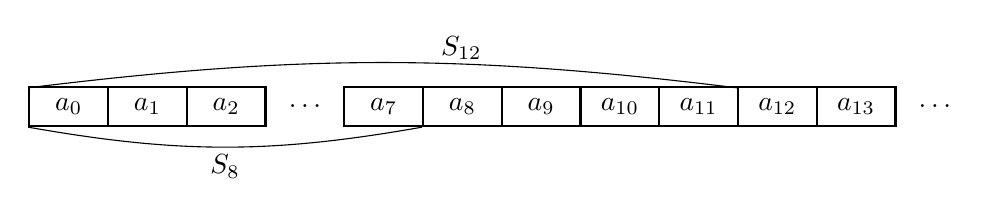
\begin{tikzpicture}[y=5mm]

\node[above right] (a0) at (0,0) [draw,thick,minimum width=1cm,minimum height=0.5cm] {$a_0$};
\node[above right] (a1) at (1,0) [draw,thick,minimum width=1cm,minimum height=0.5cm] {$a_1$};
\node[above right] (a2) at (2,0) [draw,thick,minimum width=1cm,minimum height=0.5cm] {$a_2$};
\node[above right] (a3) at (3,0) [thick,minimum width=1cm,minimum height=0.5cm] {$\ldots$};
\node[above right] (a7) at (4,0) [draw,thick,minimum width=1cm,minimum height=0.5cm] {$a_7$};
\node[above right] (a8) at (5,0) [draw,thick,minimum width=1cm,minimum height=0.5cm] {$a_8$};
\node[above right] (a9) at (6,0) [draw,thick,minimum width=1cm,minimum height=0.5cm] {$a_9$};
\node[above right] (a10) at (7,0) [draw,thick,minimum width=1cm,minimum height=0.5cm] {$a_{10}$};
\node[above right] (a11) at (8,0) [draw,thick,minimum width=1cm,minimum height=0.5cm] {$a_{11}$};
\node[above right] (a12) at (9,0) [draw,thick,minimum width=1cm,minimum height=0.5cm] {$a_{12}$};
\node[above right] (a13) at (10,0) [draw,thick,minimum width=1cm,minimum height=0.5cm] {$a_{13}$};
\node[above right] (a14) at (11,0) [thick,minimum width=1cm,minimum height=0.5cm] {$\ldots$};
\draw (0,0) to [out=-10,in=190] (5,0);
\node[] () at (2.5,-1) {$S_8$};
\draw (0,1) to [out=7,in=173] (9,1);
\node[] () at (5.5,2) {$S_{12}$};
\end{tikzpicture}
\end{center}

Using this, we can obtain the maximum value by examining the sum of all intervals.

\begin{pbox}{A Traveler}{JOI 2009}
Given a travel itinerary that goes back and forth, find the total distance walked (modulo).

\aojid{0549}
\end{pbox}

Idea: Suppose there is an instruction in the itinerary to "move to the 30th post station to the left," we want to avoid adding 30 times. Therefore, we calculate the distance from the left end for each post station in advance. Then, we can find the total distance with $M$ additions, where $M$ is the number of elements in the itinerary.

\subsection*{Two-Dimensional Cumulative Sum}

The same idea can be applied to two dimensions:
Define the auxiliary variable as $S_{i+1,j+1} = \sum_{k=0}^i \sum_{l=0}^j a_{k,l}$.
The sum of the rectangular region with vertical [i,i') and horizontal [j,j') is
$S_{i',j'} - S_{i,j'} - S_{i',j} + S_{i,j}$. (Subtract the extra from the large rectangle and adjust the over-subtracted part)
In other words, it can be found with a constant number of operations regardless of the area of the rectangular region.

\begin{center}
\begin{tikzpicture}

\draw (0,0) rectangle (6,4);
\draw[dotted] (2,0) -- (2,4);
\draw[dotted] (0,2.5) -- (6,2.5);
\node[below right] () at (0,4) [draw] {\small $a_{0,0}$};
\node[below right] () at (0,2.5) [draw] {\small $a_{i,0}$};
\node[below right] () at (2,2.5) [draw] {\small $a_{i,j}$};
\node[below right] () at (6,2.5) [draw,dotted] {\small $a_{i,j'}$};
\node[below right] () at (2,0) [draw,dotted] {\small $a_{i',j}$};
\node[below right] () at (6,0) [draw,dotted] {\small $a_{i',j'}$};
\node[] () at (1,1.25) {$C$};
\node[] () at (1,3.25) {$A$};
\node[] () at (4,1.25) {$D$};
\node[] () at (4,3.25) {$B$};
\node[] () at (10,2) {\vbox{\hbox{$A=S_{i,j}$}\hbox{$A+B=S_{i,j'}$}\hbox{$A+C=S_{i',j}$}\hbox{$A+B+C+D=S_{i',j'}$}}};
\end{tikzpicture}
\end{center}

\begin{psbox}{Maximum Sum Sequence II}{PC Koshien 2003}
Find the rectangular region with the maximum sum.

\aojid{0098}
\end{psbox}

(This problem can also be solved in $O(N^3)$ by converting it to a maximum subarray problem in either the vertical or horizontal direction. However, for the sake of the story, it is posted with the intention of solving it in $O(N^4)$ by examining all rectangular intervals.)

\begin{pbox}{Planetary Exploration}{JOI 2010}
Find the amount of resources in a specified rectangular area.

\aojid{0560}
\end{pbox}

\begin{pbox}{Coffee Central$\star$}{World Finals 2011}
Find the optimal location to open a cafe.

\url{https://icpcarchive.ecs.baylor.edu/index.php?option=com_onlinejudge&Itemid=8&category=45&page=show_problem&problem=3133}
\end{pbox}

A diamond-shaped area may be easier to handle if rotated by 45 degrees.

\section{Binary Indexed Tree (Fenwick Tree)}

Now, let's consider a situation where some of the data $a_i$ changes during processing.
If we use the auxiliary variable $S$ as in the previous section, we can answer queries in $O(1)$, which is efficient, but updates take $O(N)$. Here, we introduce a method that achieves $O(\log N)$ updates by allowing a cost of $O(\log N)$ for query responses. (\pccbook[pp. 160--])

\begin{pbox}{Range Query - Range Sum Query}{AOJ}
Manage the sum of values in a range.

\aojid{DSL_2_B}
\end{pbox}

\begin{center}
\begin{tikzpicture}[y=5mm]
\node[above right] (S8) at (0,6) [draw,thick,minimum width=8cm,minimum height=0.5cm] {$S_{1,8}$};
\node[above right] (S4) at (0,4) [draw,thick,minimum width=4cm,minimum height=0.5cm,fill=gray!15!] {$S_{1,4}$};
\node[above right] (S2) at (0,2) [draw,thick,minimum width=2cm,minimum height=0.5cm] {$S_{1,2}$};
\node[above right] (S6) at (4,2) [draw,thick,minimum width=2cm,minimum height=0.5cm,fill=gray!15!] {$S_{5,6}$};
\node[above right] (S1) at (0,0) [draw,thick,minimum width=1cm,minimum height=0.5cm] {$S_{1,1}$};
\node[above right] (S3) at (2,0) [draw,thick,minimum width=1cm,minimum height=0.5cm] {$S_{3,3}$};
\node[above right] (S5) at (4,0) [draw,thick,minimum width=1cm,minimum height=0.5cm] {$S_{5,5}$};
\node[above right] (S7) at (6,0) [draw,thick,minimum width=1cm,minimum height=0.5cm,fill=gray!15!] {$S_{7,7}$};
\node[right,color=iblue] at (7.9,6.5) {\small 8:1000};
\node[right,color=iblue] at (3.95,4.5) {\small 4:0100};
\node[right,color=iblue] at (1.95,2.5) {\small 2:0010};
\node[right,color=iblue] at (0.9,0.5) {\small 1:0001};
\node[right,color=iblue] at (5.95,2.5) {\small 6:0110};
\node[right,color=iblue] at (2.9,0.5) {\small 3:0011};
\node[right,color=iblue] at (4.9,0.5) {\small 5:0101};
\node[right,color=iblue] at (6.9,0.5) {\small 7:0111};
\end{tikzpicture}
\end{center}

First, we calculate the sum for intervals with lengths that are powers of 2, as shown in the figure. Here, the notation $S_{i,j}$ represents the sum of the interval [i,j]. This notation differs from the previous sections, and includes $j$. Also, assume that the sequence to be managed starts from $a_1$ and 1. (It is also possible to start from 0, but fine-tuning is necessary as described later).

With such preparation, $S_{1,x}$ can be expressed as the sum of up to $\log x$ terms for $x \ge 1$. For example, $S_{1,7} = S_{1,4}+S_{5,6}+S_{7,7}$.
Also, when the value of a certain element changes, it is sufficient to update at most $\log N$ partial sums. For example, when $a_7$ is updated, we update $S_{7,7}$ and $S_{1,7}$, which are the intervals that include it.

A data structure that manages such data in an array is called a Fenwick tree or Binary indexed tree (BIT). Using the element numbers (the right side of the colon is the binary representation) indicated in blue, we can manage it as follows.
The element \texttt{BIT[n]} of the $n$-th array stores the sum $S_{l,r}$ of the interval where the left end $l$ is the number obtained by dropping the lowest bit of $n$ + 1, and the right end $r$ is $n$.
Therefore, the sum from $1$ to $n$ can be obtained by first adding \texttt{BIT[n]}, and then repeating the process of finding a new interval where the right end is $l-1$ of the current interval until the left end $l$ of the covered interval reaches $1$. Such an interval can be found by dropping the lowest bit of \texttt{n}. Also, when updating $a_n$, after updating \texttt{BIT[n]}, we repeat the process of finding blocks that include that interval by expanding the right end (without reducing the left end).

\begin{cbox}
int BIT[1000010], bit_size;
void bit_init(int n) {
    fill(BIT, BIT+n, 0); 
    bit_size = n;
}
int bit_sum(int n) { // Sum of [1,n]
  int ans = 0;
  while (n > 0) { // The left end of the entire interval contains only one 1, so it ends with 0
    ans += BIT[n];
    n &= n-1; // Drop the lowest (rightmost) 1: Move to the left
  }
  return ans;
}
void bit_add(int n, int v) { // Add v to the n-th element
  while (n <= bit_size) {
    BIT[n] += v;
    n += n & (-n); // Carry up the lowest (rightmost) 1
  }
}  
\end{cbox}

\paragraph{Reference: 0-index case}
\begin{center}
\begin{tikzpicture}[y=5mm]
\node[above right] (S8) at (0,6) [draw,thick,minimum width=8cm,minimum height=0.5cm] {$S_{0,7}$};
\node[above right] (S4) at (0,4) [draw,thick,minimum width=4cm,minimum height=0.5cm] {$S_{0,3}$};
\node[above right] (S2) at (0,2) [draw,thick,minimum width=2cm,minimum height=0.5cm] {$S_{0,1}$};
\node[above right] (S6) at (4,2) [draw,thick,minimum width=2cm,minimum height=0.5cm] {$S_{4,5}$};
\node[above right] (S1) at (0,0) [draw,thick,minimum width=1cm,minimum height=0.5cm] {$S_{0,0}$};
\node[above right] (S3) at (2,0) [draw,thick,minimum width=1cm,minimum height=0.5cm] {$S_{2,2}$};
\node[above right] (S5) at (4,0) [draw,thick,minimum width=1cm,minimum height=0.5cm] {$S_{4,4}$};
\node[above right] (S7) at (6,0) [draw,thick,minimum width=1cm,minimum height=0.5cm] {$S_{6,6}$};
\node[right,color=iblue] at (7.9,6.5) {\small 7:111};
\node[right,color=iblue] at (3.95,4.5) {\small 3:011};
\node[right,color=iblue] at (1.95,2.5) {\small 1:001};
\node[right,color=iblue] at (0.9,0.5) {\small 0:000};
\node[right,color=iblue] at (5.95,2.5) {\small 5:101};
\node[right,color=iblue] at (2.9,0.5) {\small 2:010};
\node[right,color=iblue] at (4.9,0.5) {\small 4:100};
\node[right,color=iblue] at (6.9,0.5) {\small 6:110};
\end{tikzpicture}
\end{center}

\begin{itemize}
\setlength{\itemsep}{0pt}
\item[Sum:] \texttt{n = (n \& (n + 1)) - 1 } $(n\ge 0)$ Carry down the 1 with 0 to the right
\item[Update:] \texttt{n |= n + 1 } $(n<\text{size})$ Set the rightmost 0 to 1
\end{itemize}

\begin{pbox}{Moving}{Summer Camp 2012}
Find the total amount of energy required to sort in ascending order.

\aojid{2431}
\end{pbox}

Since sorting all elements is the sum from 1 to N, it is sufficient to subtract the maximum sum of the weights of the subsequences that do not need to be sorted (=ascending order).

If we denote the maximum sum of weights of ascending subsequences ending with the $i$-th number $x_i$ as $A_i$, then
$$
A_i = x_i + \max_{j<i,\, x_j<x_i} A_j
$$
Therefore, it can be obtained sequentially by looking at the sequence from the left. Here, it takes time to check the maximum value for $j$ smaller than $i$ one by one, so we use a BIT with $x_i$ as the key to process it efficiently.

\begin{cbox}
long long N, x;
int main() {
    cin >> N;
    bit_init(N+1);
    for (int i=0; i<N; ++i) {
        cin >> x;
        long long cost = // Maximum value up to x
        ... // Update the maximum value up to x to cost+x
    }
    cout << (1+N)*N/2 - bit_max(N) << endl;
}
\end{cbox}

\begin{rbox}
N = gets.to_i
X = gets.split(' ').map{|s| s.to_i}

tree = BIT_Max.new(N+1)
X.each {|x|
  cost = ... // Maximum value up to x
  ... // Update the maximum value up to x to cost+x
}
puts (1+N)*N/2 - tree.max(N)  
\end{rbox}

Instead of a BIT that manages the sum of intervals, let's consider a data structure that has the maximum value of the interval $[1,n]$ from the beginning.

\begin{cbox}
long long BIT[100010], bit_size; // long long is a 64-bit integer.
void bit_init(int n) {
    fill(BIT, BIT+n, 0); 
    bit_size = n;
}
long long bit_max(int n) { // Maximum value of [1,n]
    long long ans = 0;
    while (n > 0) {
        ans = max(ans, BIT[n]);
        n &= n-1;
    }
    return ans;
}
void bit_setmax(int n, long long v) { // Update the maximum value of [1,n] to v
    while (n < bit_size) {
        BIT[n] = max(BIT[n], v);
        n += n & (-n);
    }
}  
\end{cbox}

\begin{rbox}
class BIT_Max
  # 1-index
  def initialize(n)
    @array = Array.new(n+1, 0)
  end
  def max(n) # Maximum value of [1,n]
    ans = 0
    while n > 0
      ans = @array[n] if ans < @array[n]
      n &= n-1
    end
    ans
  end
  def setmax(n, v) # Update the maximum value of [1,n] to v
    while n < @array.size
      @array[n] = v if @array[n] < v
      n += n & (-n)
    end
  end
end
\end{rbox}
\section{Segment Tree and Range Minimum Query}\label{section:RMQ}

Next, let's consider the minimum and maximum values of intervals.
Unfortunately, the minimum value of the interval [i,j] cannot be obtained from the minimum values of the intervals [0,i] and [0,j]. Therefore, we will use a slightly richer data structure called a Segment Tree.
(\pccbook[pp.~154--]).

\begin{center}
\begin{tikzpicture}[y=5mm]
\node[above right] (S0) at (0,6) [draw,thick,minimum width=8cm,minimum height=0.5cm] {$S_{0,7}$};
\node[above right] (S1) at (0,4) [draw,thick,minimum width=3.9cm,minimum height=0.5cm] {$S_{0,3}$};
\node[above right] (S2) at (4,4) [draw,thick,minimum width=4cm,minimum height=0.5cm] {$S_{4,7}$};
\node[above right] (S3) at (0,2) [draw,thick,minimum width=1.9cm,minimum height=0.5cm] {$S_{0,1}$};
\node[above right] (S4) at (2,2) [draw,thick,minimum width=1.9cm,minimum height=0.5cm,fill=gray!15!] {$S_{2,3}$};
\node[above right] (S5) at (4,2) [draw,thick,minimum width=1.9cm,minimum height=0.5cm,fill=gray!15!] {$S_{4,5}$};
\node[above right] (S6) at (6,2) [draw,thick,minimum width=2cm,minimum height=0.5cm] {$S_{6,7}$};
\node[above right] (S7) at (0,0) [draw,thick,minimum width=.9cm,minimum height=0.5cm] {$S_{0,0}$};
\node[above right] (S8) at (1,0) [draw,thick,minimum width=.9cm,minimum height=0.5cm,fill=gray!15!] {$S_{1,1}$};
\node[above right] (S9) at (2,0) [draw,thick,minimum width=.9cm,minimum height=0.5cm] {$S_{2,2}$};
\node[above right] (S10) at (3,0) [draw,thick,minimum width=.9cm,minimum height=0.5cm] {$S_{3,3}$};
\node[above right] (S11) at (4,0) [draw,thick,minimum width=.9cm,minimum height=0.5cm] {$S_{4,4}$};
\node[above right] (S12) at (5,0) [draw,thick,minimum width=.9cm,minimum height=0.5cm] {$S_{5,5}$};
\node[above right] (S13) at (6,0) [draw,thick,minimum width=.9cm,minimum height=0.5cm,fill=gray!15!] {$S_{6,6}$};
\node[above right] (S14) at (7,0) [draw,thick,minimum width=1cm,minimum height=0.5cm] {$S_{7,7}$};
\node[color=icyan] at (7.8,6.5) {0};
\node[color=icyan] at (3.6,4.5) {1};
\node[color=icyan] at (7.8,4.5) {2};
\node[color=icyan] at (1.6,2.5) {3};
\node[color=icyan] at (3.6,2.5) {4};
\node[color=icyan] at (5.6,2.5) {5};
\node[color=icyan] at (7.8,2.5) {6};
\node[color=icyan] at (0.5,-0.5) {7};
\node[color=icyan] at (1.5,-0.5) {8};
\node[color=icyan] at (2.5,-0.5) {9};
\node[color=icyan] at (3.5,-0.5) {10};
\node[color=icyan] at (4.5,-0.5) {11};
\node[color=icyan] at (5.5,-0.5) {12};
\node[color=icyan] at (6.5,-0.5) {13};
\node[color=icyan] at (7.5,-0.5) {14};
\end{tikzpicture}
\end{center}

We maintain the data for each interval in a complete binary tree with the entire interval as the root, numbered 0 as shown in the figure. Each interval other than the leaves has two children, with the left child responsible for the left half of the parent's interval and the right child responsible for the rest.
For example, the minimum value of the interval [2,6] can be found by $\min(S_{1,2},S_{2,3},S_{4,5},S_{6,6})$, as shown in the gray area of the figure. No matter what interval is taken, the number of places to check is at most 2 for each depth.

In this implementation, for a certain \texttt{id}, the left child is \texttt{id*2+1}, the right child is \texttt{id*2+2}, and the parent is \texttt{(id-1)/2}.
If the length of the original array $a_i$ is $N$, then if $N$ is a power of 2, we use a region of $2N$, and if not, we use a region of at most $4N$.

Also, the least common ancestor (LCA) of a rooted tree can be calculated as an RMQ for the visit times of a depth-first search.
\pccbook[pp.~292--]

\begin{pbox}{Range Query - Range Minimum Query}{AOJ}
Manage the minimum value of an interval.

\aojid{DSL_2_A}
\end{pbox}

\begin{pbox}{Balanced Lineup}{USACO 2007 January Silver}
Cows are lined up. What is the difference between the tallest and shortest cows in the interval [a,b]?

\url{http://poj.org/problem?id=3264}
\end{pbox}

scanf is necessary.

\begin{pbox}{Drawing Lots$\star$}{UTPC2009}
For a lottery, find the minimum number of horizontal lines to add so that the selected location becomes a hit.

  \aojid{2192}
\end{pbox}

\begin{pbox}{Distance Queries$\star$}{USACO 2004 February}

Find the distance between two points on a farm.

\url{http://poj.org/problem?id=1986}
\end{pbox}


\begin{pbox}{Apple Tree$\star$}{POJ Monthly--2007.08.05}

Count the number of apples.

\url{http://poj.org/problem?id=3321}
\end{pbox}
\chapter{Stable Matching (Stable Marriage Problem)}

Consider the problem of matching elements between two groups, A and B. Examples include matching medical residents with hospitals, marriages between men and women, and products with factories. We will first address the problem where A and B have the same number of elements, $N$, and we create $N$ pairs by selecting one element from A and one from B, ensuring no element is repeated (a \textbf{matching}\footnote{In graph theory, a set of edges that are not adjacent to each other (i.e., \textbf{independent}) is called a \textbf{matching}.}).

For example, if the theme is marriage, A and B would be men and women. Here, we assume that each individual has a list showing their preference ranking for potential partners, and the list includes all members of the opposite sex. In this setting, it is possible to create stable pairs that satisfy everyone's preferences in a certain sense. Here, stability means that there is *no* situation where "a man and a woman would both prefer to break their current pairs and form a new pair."

\begin{itembox}{Examples of Stable and Unstable Pairs}
  Suppose that job types $A$ and $B$ are recruiting one person each, and applicants $a$ and $b$ have each determined their preference rankings. In the following examples, if $Aa$ is not paired, then breaking the current pairs and forming the pair $Aa$ would result in both $A$ and $a$ being in a more desirable situation than their current pairs.

  \begin{center}
  \begin{tabular}{cccc|lll}
    \multicolumn{4}{l|}{Preference Ranking} & Stable & Unstable & Reason for Instability\\
    $A$ & $B$ & $a$ & $b$ \\\hline
    $ab$&  $ba$& $AB$& $BA$   & ($Aa, Bb$) & ($Ab, Ba$) & First choices match\\
    $ab$&  $ab$& $AB$& $BA$   & ($Aa, Bb$) & ($Ab, Ba$)
    & $B$ prefers $a$ but is unstable\\
    $ab$&  $ab$& $AB$& $AB$   & ($Aa, Bb$) & ($Ab, Ba$)& $B$ and $b$ prefer each other but is unstable
  \end{tabular}
  \end{center}
\end{itembox}

This problem can be solved by repeatedly (1) determining temporary pairs and (2) replacing them with higher-priority pairs that are formed later (Gale–Shapley).
\begin{cbox}
while not everyone is paired
  Select a single unmarried man, m
  Let f be the highest-ranked woman on m's preference list who has not yet rejected m
  if f is unmarried
    Pair m and f
  else if f is currently paired with m'
    if f prefers m' to m
      m remains unmarried
    else
      Pair m and f
      m' becomes unmarried
    end
  end
end
\end{cbox}

\medskip

This problem can be solved by repeatedly (1) determining temporary pairs and (2) replacing them with higher-priority pairs that are formed later. Since men and women are symmetrical, a stable solution can be obtained even if they are swapped. In that case, the difference appears in which side's preferences are prioritized when there are multiple stable solutions. To shorten the notation, we denote the state of not having a pair as unmarried.

\begin{pbox}{The Stable Marriage Problem}{Southeastern Europe 2007}

Given the preference lists of $N$ men and $N$ women, create a stable matching that prioritizes the men's preferences.

Men are represented by a single uppercase letter, and women are represented by a single lowercase letter. Each preference list contains $N$ people. The output should be processed in the order of the men's names.

\url{http://poj.org/problem?id=3487}
\end{pbox}

Since each man and woman is given by name, it is slightly more complex than when given by numbers such as 0..N.
Here, we use the fact that a single alphabet character is equivalent to a numerical value in the range $[0,127]$ and treat it as a number.
The preference list of man \texttt{'a'} is represented by the first $N$ characters of \texttt{pref\_m['a']}, and similarly, the preference list of woman \texttt{'A'} is represented by \texttt{pref\_m['A']}.
That is, for man \texttt{'a'}, the most preferred woman is \texttt{pref\_m['a'][0]}, the next is \texttt{pref\_m['a'][1]}, and so on.
The unused parts of the table are filled with NULL characters (automatically converted from 0 in C++).

\begin{cbox}
#include <algorithm>
// In the first sample, pref\_m['a'] is BAC... (only the first N characters are used, others are null)
char pref_m[256][256]={{0}}, pref_f[256][256]={{0}};

// Returns true if woman f prefers man a to man b
bool better(char f, char a, char b) {
  int orda = find(pref_f[f], pref_f[f]+27, a) - pref_f[f]; // Rank of a in the list
  int ordb = find(pref_f[f], pref_f[f]+27, b) - pref_f[f]; // Rank of b
  return orda < ordb;
}
\end{cbox}

Next, create the input/output. It is a bit complex, so even if you do not understand every detail of the following sample, it is okay if you can confirm that it works. \texttt{scanf(" \%c",c)} is a syntax that skips whitespace and reads one character.

\begin{cbox}
#include <cstdio>
#include <iostream>
#include <string>
using namespace std;
int T, N;
int main() {
    scanf("%d", &T);
    for (int t=0; t<T; ++t) {
        scanf("%d", &N);
        string name_m, name_f;
        char c;
        for (int i=0; i<N; ++i) {
            scanf(" %c", &c);
            name_m += c;
        }
        for (int i=0; i<N; ++i) {
            scanf(" %c", &c);
            name_f += c;
        }
        sort(name_m.begin(), name_m.end());
        
        for (int i=0; i<N; ++i) {
            scanf(" %c:", &c);
            scanf(" %s", pref_m[c]);
        }
        for (int i=0; i<N; ++i) {
            scanf(" %c:", &c);
            scanf(" %s", pref_f[c]);
        }
        if (t>0) puts("");
        // Before solving the problem, let's output pref\_m and pref\_f
        for (int i=0; i<N; ++i)
            cout << name\_m[i] << pref\_m[name\_m[i]] << endl;
        for (int i=0; i<N; ++i)
            cout << name\_f[i] << pref\_f[name\_f[i]] << endl;
        // Then combine it to call the solve() function around here
    }
}
\end{cbox}

\begin{center}
  \begin{tabular}{l@{\hspace{1.5cm}}l@{\hspace{1.5cm}}l}
      \begin{tikzpicture}[node distance=15mm]
        \node[city] (a)              {$a$};
        \node[city] (b) [right of=a] {$b$};
        \node[city] (c) [right of=b] {$c$};

        \node[city] (A) [below of=a] {$A$};
        \node[city] (B) [right of=A] {$B$};
        \node[city] (C) [right of=B] {$C$};

        \path[->,thick,draw=red] (a) edge (B);
      \end{tikzpicture}
&
      \begin{tikzpicture}[node distance=15mm]
        \node[city] (a)              {$a$};
        \node[city] (b) [right of=a] {$b$};
        \node[city] (c) [right of=b] {$c$};

        \node[city] (A) [below of=a] {$A$};
        \node[city] (B) [right of=A] {$B$};
        \node[city] (C) [right of=B] {$C$};

        \path[->,thick] (a) edge (B);
        \path[->,dotted,draw=red] (b) edge (B);
      \end{tikzpicture}

&
      \begin{tikzpicture}[node distance=15mm]
        \node[city] (a)              {$a$};
        \node[city] (b) [right of=a] {$b$};
        \node[city] (c) [right of=b] {$c$};

        \node[city] (A) [below of=a] {$A$};
        \node[city] (B) [right of=A] {$B$};
        \node[city] (C) [right of=B] {$C$};

        \path[->,thick,draw=red] (b) edge (B);
      \end{tikzpicture}
\\
(1) a's first choice is B & (2) b's first choice is B (conflict) & (3) B prefers b to a \\
      \begin{tikzpicture}[node distance=15mm]
        \node[city] (a)              {$a$};
        \node[city] (b) [right of=a] {$b$};
        \node[city] (c) [right of=b] {$c$};

        \node[city] (A) [below of=a] {$A$};
        \node[city] (B) [right of=A] {$B$};
        \node[city] (C) [right of=B] {$C$};

        \path[->,thick,draw=red] (a) edge (A);
        \path[->,thick] (b) edge (B);
      \end{tikzpicture}
&
      \begin{tikzpicture}[node distance=15mm]
        \node[city] (a)              {$a$};
        \node[city] (b) [right of=a] {$b$};
        \node[city] (c) [right of=b] {$c$};

        \node[city] (A) [below of=a] {$A$};
        \node[city] (B) [right of=A] {$B$};
        \node[city] (C) [right of=B] {$C$};

        \path[->,thick] (a) edge (A);
        \path[->,thick] (b) edge (B);
        \path[->,dotted,draw=red] (c) edge (A);
      \end{tikzpicture}
&
      \begin{tikzpicture}[node distance=15mm]
        \node[city] (a)              {$a$};
        \node[city] (b) [right of=a] {$b$};
        \node[city] (c) [right of=b] {$c$};

        \node[city] (A) [below of=a] {$A$};
        \node[city] (B) [right of=A] {$B$};
        \node[city] (C) [right of=B] {$C$};

        \path[->,thick] (a) edge (A);
        \path[->,thick] (b) edge (B);
        \path[->,thick,draw=red] (c) edge (C);
      \end{tikzpicture}
\\
(4) a's next choice is A & (5) c also prefers A (conflict) & (6) A chooses a and c goes to C
  \end{tabular}
The Stable Marriage Problem: Example of operation in the first sample
\end{center}

Next, implement the algorithm.
The current pair of man \texttt{'a'} is represented by \texttt{m2f['a']} (NULL character if not present).
Similarly, the current pair of woman \texttt{'A'} is represented by \texttt{f2m['A']}.

The number of women that man \texttt{'a'} has proposed to in his list is managed by \texttt{proposed['a']}.

\begin{cbox}
void solve(string name_m, string name_f) {
    char m2f[256]={0}, f2m[256]={0};
    int proposed[256]={0};
    int man_id = 0; // Index of the man
    while (true) {
        char man = name_m[man_id]; // Name of the man
        if (m2f[man]) { // Already assigned
            ++man_id; // Move to the next person
            if (man_id == N) break;
            continue;
        }
        // man does not have a pair yet
        while (!m2f[man]) {
            char f =  pref_m[man][proposed[man]]; // Select the woman of "next priority" for man
            proposed[man]++; // Increment the "next priority" of man
            char mate = f2m[f]; // Current pair of f
            if (! mate || better(f, man, mate)) {
                if (mate) m2f[mate] = 0; // Cancel the pair of mate and f
                m2f[man] = f; // Record the pair of man and f in m2f
                f2m[f] = man; // Record the pair of man and f in f2m
                man_id = 0; // Start over from the beginning
            }
        }
    }
    for (int i=0; i<N; ++i)
        printf("%c %c\n", name_m[i], m2f[name_m[i]]);
}
\end{cbox}

\chapter{Bipartite Graph Matching}

Let's consider the problem of finding a maximum matching in a bipartite graph. This problem is similar to the previous section, but differs in that there are no preference rankings and it is not guaranteed that everyone can be paired. Determining temporary pairs and reassigning them as needed is similar to the previous section, but the decision of whether or not to reassign requires recursion. (\pccbook[pp.~195--])

\begin{psbox}{Matching - Bipartite Matching}{AOJ}
  
\aojid{GRL_7_A}
\end{psbox}

An example of the operation with sample input 1 is shown below.

\begin{center}
  \begin{tabular}{l@{\hspace{1.5cm}}l}
      \begin{tikzpicture}[node distance=15mm]
        \node[city] (a)              {$0$};
        \node[city] (b) [right of=a] {$1$};
        \node[city] (c) [right of=b] {$2$};

        \node[city] (A) [below of=a] {$0$};
        \node[city] (B) [right of=A] {$1$};
        \node[city] (C) [right of=B] {$2$};
        \node[city] (D) [right of=C] {$3$};

        \path[draw=gray,thick] (a) edge (A);
        \path[draw=gray,thick] (a) edge (C);
        \path[draw=gray,thick] (a) edge (D);
        \path[draw=gray,thick] (b) edge (B);
        \path[draw=gray,thick] (c) edge (B);
        \path[draw=gray,thick] (c) edge (C);
      \end{tikzpicture}
&
      \begin{tikzpicture}[node distance=15mm]
        \node[vcity] (a)              {$0$};
        \node[city] (b) [right of=a] {$1$};
        \node[city] (c) [right of=b] {$2$};

        \node[ccity] (A) [below of=a] {$0$};
        \node[city] (B) [right of=A] {$1$};
        \node[city] (C) [right of=B] {$2$};
        \node[city] (D) [right of=C] {$3$};

        \path[draw=red,thick] (a) edge (A);
        \path[draw=gray,thick] (a) edge (C);
        \path[draw=gray,thick] (a) edge (D);
        \path[draw=gray,thick] (b) edge (B);
        \path[draw=gray,thick] (c) edge (B);
        \path[draw=gray,thick] (c) edge (C);
      \end{tikzpicture}\\
  Initial state & Create a temporary pair from 0 above\\
      \begin{tikzpicture}[node distance=15mm]
        \node[vcity] (a)              {$0$};
        \node[vcity] (b) [right of=a] {$1$};
        \node[city] (c) [right of=b] {$2$};

        \node[ccity] (A) [below of=a] {$0$};
        \node[ccity] (B) [right of=A] {$1$};
        \node[city] (C) [right of=B] {$2$};
        \node[city] (D) [right of=C] {$3$};

        \path[draw=blue,thick] (a) edge (A);
        \path[draw=gray,thick] (a) edge (C);
        \path[draw=gray,thick] (a) edge (D);
        \path[draw=red,thick] (b) edge (B);
        \path[draw=gray,thick] (c) edge (B);
        \path[draw=gray,thick] (c) edge (C);
      \end{tikzpicture}
&
      \begin{tikzpicture}[node distance=15mm]
        \node[vcity] (a)              {$0$};
        \node[vcity] (b) [right of=a] {$1$};
        \node[vcity] (c) [right of=b] {$2$};

        \node[ccity] (A) [below of=a] {$0$};
        \node[ccity] (B) [right of=A] {$1$};
        \node[city] (C) [right of=B] {$2$};
        \node[city] (D) [right of=C] {$3$};

        \path[draw=blue,thick] (a) edge (A);
        \path[draw=gray,thick] (a) edge (C);
        \path[draw=gray,thick] (a) edge (D);
        \path[draw=blue,thick] (b) edge (B);
        \path[draw=red,thick] (c) edge (B);
        \path[draw=gray,thick] (c) edge (C);
      \end{tikzpicture}\\
Create a temporary pair from 1 above & A conflict occurs when trying to create a temporary pair from 2 above
\\
      \begin{tikzpicture}[node distance=15mm]
        \node[vcity] (a)              {$0$};
        \node[vcity] (b) [right of=a] {$1$};
        \node[city] (c) [right of=b] {$2$};

        \node[ccity] (A) [below of=a] {$0$};
        \node[ccity] (B) [right of=A] {$1$};
        \node[city] (C) [right of=B] {$2$};
        \node[city] (D) [right of=C] {$3$};

        \path[draw=blue,thick] (a) edge (A);
        \path[draw=gray,thick] (a) edge (C);
        \path[draw=gray,thick] (a) edge (D);
        \path[draw=blue,dotted] (b) edge (B);
        \path[draw=red,thick] (c) edge (B);
        \path[draw=gray,thick] (c) edge (C);
      \end{tikzpicture}
&
      \begin{tikzpicture}[node distance=15mm]
        \node[vcity] (a)              {$0$};
        \node[vcity] (b) [right of=a] {$1$};
        \node[vcity] (c) [right of=b] {$2$};

        \node[ccity] (A) [below of=a] {$0$};
        \node[ccity] (B) [right of=A] {$1$};
        \node[city] (C) [right of=B] {$2$};
        \node[city] (D) [right of=C] {$3$};

        \path[draw=blue,thick] (a) edge (A);
        \path[draw=gray,thick] (a) edge (C);
        \path[draw=gray,thick] (a) edge (D);
        \path[draw=blue,thick] (b) edge (B);
        \path[draw=gray,dotted] (c) edge (B);
        \path[draw=red,thick] (c) edge (C);
      \end{tikzpicture}\\
Even if 1's pair is rearranged, 1 above is isolated & Return 1's temporary pair and 2 makes a different pair
  \end{tabular}
\end{center}

Let's also check a slightly more complex example where reassignment occurs.
\begin{alltt}
3 3 6
0 0
0 1
0 2
1 0
1 1
2 0
\end{alltt}

\begin{center}
  \begin{tabular}{l@{\hspace{1.5cm}}l@{\hspace{1.5cm}}l}
      \begin{tikzpicture}[node distance=15mm]
        \node[city] (a)              {$0$};
        \node[city] (b) [right of=a] {$1$};
        \node[city] (c) [right of=b] {$2$};

        \node[city] (A) [below of=a] {$0$};
        \node[city] (B) [right of=A] {$1$};
        \node[city] (C) [right of=B] {$2$};

        \path[draw=gray,thick] (a) edge (A);
        \path[draw=gray,thick] (a) edge (B);
        \path[draw=gray,thick] (a) edge (C);
        \path[draw=gray,thick] (b) edge (A);
        \path[draw=gray,thick] (b) edge (B);
        \path[draw=gray,thick] (c) edge (A);
      \end{tikzpicture}
      &
      \begin{tikzpicture}[node distance=15mm]
        \node[vcity] (a)              {$0$};
        \node[city] (b) [right of=a] {$1$};
        \node[city] (c) [right of=b] {$2$};

        \node[ccity] (A) [below of=a] {$0$};
        \node[city] (B) [right of=A] {$1$};
        \node[city] (C) [right of=B] {$2$};

        \path[draw=red,thick] (a) edge (A);
        \path[draw=gray,thick] (a) edge (B);
        \path[draw=gray,thick] (a) edge (C);
        \path[draw=gray,thick] (b) edge (A);
        \path[draw=gray,thick] (b) edge (B);
        \path[draw=gray,thick] (c) edge (A);
      \end{tikzpicture}
&
      \begin{tikzpicture}[node distance=15mm]
        \node[vcity] (a)              {$0$};
        \node[vcity] (b) [right of=a] {$1$};
        \node[city] (c) [right of=b] {$2$};

        \node[ccity] (A) [below of=a] {$0$};
        \node[city] (B) [right of=A] {$1$};
        \node[city] (C) [right of=B] {$2$};

        \path[draw=red,thick] (a) edge (A);
        \path[draw=gray,thick] (a) edge (B);
        \path[draw=gray,thick] (a) edge (C);
        \path[draw=red,thick] (b) edge (A);
        \path[draw=gray,thick] (b) edge (B);
        \path[draw=gray,thick] (c) edge (A);
      \end{tikzpicture}\\
  Initial state & Create a temporary pair from 0 above & 1's temporary pair above is $\cdots$\\
      \begin{tikzpicture}[node distance=15mm]
        \node[vcity] (a)              {$0$};
        \node[vcity] (b) [right of=a] {$1$};
        \node[city] (c) [right of=b] {$2$};

        \node[ccity] (A) [below of=a] {$0$};
        \node[ccity] (B) [right of=A] {$1$};
        \node[city] (C) [right of=B] {$2$};

        \path[draw=red,dotted] (a) edge (A);
        \path[draw=red,thick] (a) edge (B);
        \path[draw=gray,thick] (a) edge (C);
        \path[draw=red,thick] (b) edge (A);
        \path[draw=gray,thick] (b) edge (B);
        \path[draw=gray,thick] (c) edge (A);
      \end{tikzpicture}
&
      \begin{tikzpicture}[node distance=15mm]
        \node[vcity] (a)              {$0$};
        \node[vcity] (b) [right of=a] {$1$};
        \node[vcity] (c) [right of=b] {$2$};

        \node[ccity] (A) [below of=a] {$0$};
        \node[ccity] (B) [right of=A] {$1$};
        \node[city] (C) [right of=B] {$2$};

        \path[draw=red,dotted] (a) edge (A);
        \path[draw=red,thick] (a) edge (B);
        \path[draw=gray,thick] (a) edge (C);
        \path[draw=red,thick] (b) edge (A);
        \path[draw=gray,thick] (b) edge (B);
        \path[draw=red,thick] (c) edge (A);
      \end{tikzpicture}
&
      \begin{tikzpicture}[node distance=15mm]
        \node[vcity] (a)              {$0$};
        \node[vcity] (b) [right of=a] {$1$};
        \node[vcity] (c) [right of=b] {$2$};

        \node[ccity] (A) [below of=a] {$0$};
        \node[ccity] (B) [right of=A] {$1$};
        \node[city] (C) [right of=B] {$2$};

        \path[draw=red,dotted] (a) edge (A);
        \path[draw=red,dotted] (a) edge (B);
        \path[draw=gray,thick] (a) edge (C);
        \path[draw=red,dotted] (b) edge (A);
        \path[draw=red,thick] (b) edge (B);
        \path[draw=red,thick] (c) edge (A);
      \end{tikzpicture}\\
Reassign the temporary pair of 0 above & 2's temporary pair is & Reassign 0 below\\
      \begin{tikzpicture}[node distance=15mm]
        \node[vcity] (a)              {$0$};
        \node[vcity] (b) [right of=a] {$1$};
        \node[vcity] (c) [right of=b] {$2$};

        \node[ccity] (A) [below of=a] {$0$};
        \node[ccity] (B) [right of=A] {$1$};
        \node[city] (C) [right of=B] {$2$};

        \path[draw=red,dotted] (a) edge (A);
        \path[draw=red,dotted] (a) edge (B);
        \path[draw=gray,thick] (a) edge (C);
        \path[draw=red,dotted] (b) edge (A);
        \path[draw=red,thick] (b) edge (B);
        \path[draw=red,thick] (c) edge (A);
      \end{tikzpicture}
&
      \begin{tikzpicture}[node distance=15mm]
        \node[vcity] (a)              {$0$};
        \node[vcity] (b) [right of=a] {$1$};
        \node[vcity] (c) [right of=b] {$2$};

        \node[ccity] (A) [below of=a] {$0$};
        \node[ccity] (B) [right of=A] {$1$};
        \node[city] (C) [right of=B] {$2$};

        \path[draw=red,dotted] (a) edge (A);
        \path[draw=red,dotted] (a) edge (B);
        \path[draw=red,thick] (a) edge (C);
        \path[draw=red,dotted] (b) edge (A);
        \path[draw=red,thick] (b) edge (B);
        \path[draw=red,thick] (c) edge (A);
      \end{tikzpicture}\\
Reassign 1 above & Reassign 0 above & 
  \end{tabular}
\end{center}

Input example
\begin{cbox}
int X, Y, E, x, y; // Problem input
bool D[110][110] = {}; // Adjacency matrix
int main() {
  cin >> X >> Y >> E;
  for (int i=0; i<E; ++i) {
    cin >> x >> y;
    D[x][y] = true;
  }
  // Calculate here
}
\end{cbox}

Calculation part
\begin{cbox}
int PY[110]; // Current pair of Y
bool V[110];
bool match(int x) {
  if (x<0) return true;
  if (V[x]) return false;
  V[x] = true;
  for (int y=0; y<Y; ++y) {
    if (!D[x][y]) continue;
    if (match(PY[y])) {
      PY[y] = x;
      return true;
    }
  }
  return false;
}
int main() {
  ... // Assume input is finished
  fill(PY, PY+Y, -1); // Initialize current pairs
  int count = 0; // Number of matches
  for (int x=0; x<X; ++x) { // Try sequentially from the X side
    fill(V, V+X, false);
    if (match(x)) ++count; // If at least one assignment starting from x succeeds
  }
  ... // Output
}
\end{cbox}

\begin{pbox}{Cards$\star$}{National Preliminary 2009}

Pair blue and red cards and remove them. What is the maximum number that can be removed?
  
\aojid{1163}
\end{pbox}

\begin{cbox}
int main() {
    while (input) {
       // Set all red card pairs to none (-1)
       P[all red] = -1;
       // C[blue][red]=1 (if pairable), C[blue][red]=0 (if not pairable)
       setting
       for (all blue cards: blue)
           for (all red cards: red)
               C[blue][red] = (__gcd(B[blue], R[red]) >= 2);
       // Match one blue card at a time
       count = 0;
       for (all blue cards: blue) {
           V[all red] = false;
           if (match(blue)) ++count;
       }
       count is the answer;
    }
}
\end{cbox}

\begin{cbox}
// V[red] .. true if card red has no new assignment, false if unknown
// P[red] .. blue card number paired with card red, -1 if no assignment
bool match(int blue) { // Can blue be paired without reducing the number of pairs so far?
    if (blue < 0) return true;
    for (all red cards: red) {
       if (``blue'' and ``red'' cannot be paired || V[red] is true) continue;
       V[red] = true;
       if (match(P[red])) { // If a different pair can be found for P[red]
         P[red] = blue; // The new pair of ``red'' is blue
         return true;
       }
    }
    return false;
}
\end{cbox}

\begin{pbox}{Defend the Bases$\star$}{Summer Camp 2009}
Move the troops and defend all the bases. (Although not specified, it seems that there are enough troops)
  
\aojid{2161}
\end{pbox}
\section{Various Matchings}

\begin{pbox}{Skiers$\star$}{9th Polish Olympiad in Informatics}
Find the minimum number of times you need to climb to the top to inspect all the courses in a ski resort.

\url{http://main.edu.pl/en/archive/oi/9/nar}
\end{pbox}

\begin{pbox}{Dangerous Tower}
I want to build a tall tower.
\aojid{2293}
\end{pbox}

\begin{pbox}{Travel Agency$\star\star$}{Algorithmic Engagements 2006}
People who want to travel together and people who don't want to travel together (!) are modeled numerically.
Find the optimal travel members.

\url{http://main.edu.pl/en/archive/pa/2006/biu}
\end{pbox}

\begin{pbox}{Matching$\star\star$}{Central European Olympiad in Informatics 2011}
Select a series of buildings where a series of logos can be placed.

\url{http://main.edu.pl/en/archive/ceoi/2011/mat}
\end{pbox}

This problem is closer to string matching.

\begin{pbox}{Ice Skates}{}
Assignment of ice skates.

\url{http://main.edu.pl/en/archive/oi/16/lyz}
\end{pbox}
\chapter{Combinatorial Games}

\section{Impartial Games}

Some combinatorial games seem to have relatively frequent examples in problem sets. For some games, such as the solution to Nim, Grundy numbers (\pccbook[pp.~272--]), and surreal numbers (\url{https://www.youtube.com/watch?v=Us8UDUqgiLo}), it is possible to efficiently determine the overall winner by analyzing subgames. Subgames correspond to situations where moves in one part do not affect other parts, such as the piles in Nim or the endgame in Go (after the major life-and-death situations have been decided). For more detailed information, see, for example, \url{http://www.math.ucla.edu/~tom/Game_Theory/Contents.html}.

\begin{psbox}[Nim (Stanford Local 2005)]
For a given situation, find the number of winning moves.
  
\url{http://poj.org/problem?id=2975}
\end{psbox}

\begin{pbox}[Christmas Game (POJ Founder Monthly Contest 2008.12.28)]

A two-player game. There is a graph that is roughly a rooted forest: cycles only exist at the ends, and the cycles do not share edges. A single move is "cut one edge and discard the subgraph on the side that is not connected to the root." (There may be two-sided polygons, etc.).

\url{http://poj.org/problem?id=3710} 
\end{pbox}

\begin{pbox}[Chef Game (November Long Challenge 2013)]
Consider a game where numbers are stacked in piles, and players choose numbers (odd or even) that they are responsible for and remove them and everything after.

Answer whether the first player should choose even or odd numbers, or neither.

\url{http://www.codechef.com/NOV13/problems/CHEFGM/}
\end{pbox}

\begin{pbox}[Unfair Game (Spring Camp 2014)]
Nim where the upper limit of the number that can be removed differs depending on the player.

\url{http://jag2014spring.contest.atcoder.jp/tasks/icpc2014spring_j}
\end{pbox}

\section{Problems Solved by Exhaustive Search}

\begin{psbox}[Aaron and Bruce]
  Given a graph, find how many turns (or infinite) A(aron) and B(ruce) can continue to escape when moving alternately.

\aojid{2108}
\end{psbox}

\begin{pbox}[House of Cards (World Finals 2009)]
Play a game of stacking cards. Who is the winner?

\url{https://icpcarchive.ecs.baylor.edu/index.php?option=com_onlinejudge&Itemid=8&category=43&page=show_problem&problem=2452}  
\end{pbox}

Data Supplement
\begin{alltt}
Axel
13
1R 2R 3R 4R 5R 6R 7R 8R 9R 10R 11R 12R 13R 1B 2B 3B 4B 5B 6B 7B 8B 9B 10B 11B 12B 13B
Case 1: Axel loses 30
\end{alltt}

\centerline{\includegraphics[width=0.9\linewidth]{gametreekr.eps}}


\begin{itemize}
\item Explanation of min-max tree \url{http://en.wikipedia.org/wiki/Minimax}
\item There are cases where it is appropriate to go back from solved states (Retrograde analysis, c.f., complete analysis of Dobutsu Shogi) and
\item cases where it is more appropriate to investigate the future from the state you want to solve (search + $\alpha-\beta$ pruning, etc.). $\alpha-\beta$ pruning is most efficient when reading in order from the best move, and the number of search nodes becomes about the square root of the case where all are read. \url{http://en.wikipedia.org/wiki/Alpha}
\end{itemize}

Various things
\begin{itemize}
\item Representation of the state: If the state (situation) is represented in a small way, copying is easy. Breadth-first and best-first searches are also possible. If you use a large representation, prepare one globally and makemove/unmake move. Only depth-first search is suitable. If necessary, do iterative deepening.
\item How to create an evaluation function: Easy for games that increase the sum of numbers like the above ``House of Cards''. Evaluation functions for Othello and Shogi are created statistically from a large amount of data, so they probably won't appear in short contests.
\item Pay attention to merges and loops: In most games, the game "tree" is not a tree. When handling merges, a state table (transposition table, in short, a dp table) is required. Loops make the story even more complicated. Especially when the history affects the outcome (a draw on the 4th occurrence of the same state, but the attacker loses in the case of repeated continuous checks, or Ko in Go), if the effect of the history is not considered when writing the outcome in the state table, the outcome may be incorrect (GHI, graph history interaction problem). If possible, Retrograde analysis is safer.
\end{itemize}

Other:
\begin{itemize}
\item Monte Carlo tree search (MCTS, UCT) Probably won't appear in short contests? \url{http://en.wikipedia.org/wiki/Monte_Carlo_tree_search}
\item Proof-number search: A type of best-first search that expands from where it seems necessary for proof \url{http://webdocs.cs.ualberta.ca/~mmueller/ps/ICGA2012PNS.pdf},
  \url{http://web.archive.org/web/20041204235835/http://www.cs.vu.nl/~victor/thesis.html}
\end{itemize}

\section{Other Problems}

\begin{pbox}[Ononokomachi's Edit War]
Mathematical expression editing game.

\aojid{2512}
\end{pbox}

\begin{pbox}[Chat noir (UTPC 2009)]
Can the cat escape?
  
\aojid{2196}
\end{pbox}

\begin{pbox}[Game Strategy (World Finals 2014)]
Alice and Bob's game.

\url{https://icpcarchive.ecs.baylor.edu/index.php?option=com_onlinejudge&Itemid=8&category=590&page=show_problem&problem=4785}
\end{pbox}

\begin{pbox}[Iyasugigappa]
A game for three people (?) : Frog, Kappa, and Weasel.

\aojid{2557}
\end{pbox}

\begin{pbox}[Sweet War]
A two-player game where players eat or pass chocolates at the beginning of a sequence. Determine the winner.

\aojid{1353}
\end{pbox}

\begin{pbox}[Circular Game]
Players move pieces in turns; the player who cannot move loses. Who wins?

\url{http://main.edu.pl/en/archive/pa/2009/gra}
\end{pbox}

\begin{pbox}[Termites]
A sequence of numbers is given. Players A and B take turns adding a number adjacent to a 0 in the sequence to their score and changing that number to 0. Find the scores of both players when they play optimally.

\url{http://main.edu.pl/en/archive/pa/2010/ter}
\end{pbox}

It is probably safer to use scanf.
